\documentclass[11pt, twocolumn]{article}
\usepackage{cite}

\usepackage{hyperref}
%biblio
\usepackage{natbib}
\usepackage{url}
\usepackage{wrapfig}

%Math
\usepackage{amsmath}
\usepackage{amsfonts}
\usepackage{amssymb}
\usepackage{amsthm}
\usepackage{ulem}
\usepackage{bm}
\usepackage{stmaryrd} %f\UTF{00FC}r Blitz!

%PageStyle
%\usepackage[ngerman]{babel} % deutsche Silbentrennung1
\usepackage[utf8x]{inputenc} 
\usepackage{fancyhdr, graphicx}
\usepackage{subcaption}
\usepackage[scaled=0.92]{helvet}
\usepackage{enumitem}
\usepackage{parskip}
\usepackage[a4paper,top=2cm]{geometry}
\setlength{\textwidth}{17cm}
\setlength{\oddsidemargin}{-0.5cm}
\usepackage{lastpage} % for getting last page number
\renewcommand{\familydefault}{\sfdefault}
\usepackage{setspace}
\usepackage{acronym}
%\usepackage[english]{babel}

\usepackage{multicol}
\setlength{\columnsep}{1cm}



% Code listenings
\usepackage{color}
\usepackage{xcolor}
\usepackage{listings}
\usepackage[font=it]{caption}
\DeclareCaptionFont{white}{\color{white}}
\DeclareCaptionFormat{listing}{\colorbox{gray}{\parbox{\textwidth}{#1#2#3}}}
\captionsetup[lstlisting]{format=listing,labelfont=white,textfont=white}
\lstset{
 language=Java,
 basicstyle=\footnotesize\ttfamily, % Standardschrift
 numbers=left,               % Ort der Zeilennummern
 numberstyle=\tiny,          % Stil der Zeilennummern
 stepnumber=1,              % Abstand zwischen den Zeilennummern
 numbersep=5pt,              % Abstand der Nummern zum Text
 tabsize=2,                  % Groesse von Tabs
 extendedchars=true,         %
 breaklines=true,            % Zeilen werden Umgebrochen
 frame=b,         
 %commentstyle=\itshape\color{LightLime}, Was isch das? O_o
 %keywordstyle=\bfseries\color{DarkPurple}, und das O_o
 basicstyle=\small,
 stringstyle=\color[RGB]{42,0,255}\ttfamily, % Farbe der String
 keywordstyle=\color[RGB]{127,0,85}\ttfamily, % Farbe der Keywords
 commentstyle=\color[RGB]{63,127,95}\ttfamily, % Farbe des Kommentars
 showspaces=false,           % Leerzeichen anzeigen ?
 showtabs=false,             % Tabs anzeigen ?
 xleftmargin=17pt,
 framexleftmargin=17pt,
 framexrightmargin=5pt,
 framexbottommargin=4pt,
 showstringspaces=false      % Leerzeichen in Strings anzeigen ?        
}

\usepackage{xcolor}

%Config
\fancypagestyle{firststyle}{ %Style of the first page
 \fancyhf{}
 \fancyheadoffset[L]{0.6cm}
 \lhead{
 
\includegraphics[scale=0.8]{./fhnw_ht_e_10mm.jpg}}
 \renewcommand{\headrulewidth}{0pt}
 \lfoot{Institute 4 Data Science,\linebreak www.fhnw.ch }
}

\fancypagestyle{documentstyle}{ %Style of the rest of the document
 \fancyhf{}
 \fancyheadoffset[L]{0.6cm}
\lhead{
 
\includegraphics[scale=0.8]{./fhnw_ht_e_10mm.jpg}}
 \renewcommand{\headrulewidth}{0pt}
 \lfoot{P9 Distributed Image Reconstruction for new Radio Interferometers}
 \rfoot{\thepage\ / \pageref{LastPage} }
}

\fancypagestyle{tableofcontent}{ %Style of the rest of the document
 \fancyhf{}
 \fancyheadoffset[L]{0.6cm}
\lhead{
 
\includegraphics[scale=0.8]{./fhnw_ht_e_10mm.jpg}}
 \renewcommand{\headrulewidth}{0pt}
 \cfoot{\thepage}
}

\fancypagestyle{abstract}{ %Style of the first page
 \fancyhf{}
 \fancyheadoffset[L]{0.6cm}
 \lhead{
 
\includegraphics[scale=0.8]{./fhnw_ht_e_10mm.jpg}}
 \renewcommand{\headrulewidth}{0pt}
 \cfoot{}
}


%Metadata
\numberwithin{equation}{section}

\newlength{\twosubht}
\newsavebox{\twosubbox}

\begin{document}
\title{P9 Distributed Image Reconstruction for the new Radio Interferometers}
\author{Jonas Schwammberger}
\date{\today}
\begin{titlepage}
	\maketitle
	
	%\begin{figure}[h]
	%	\centering
	%	\includegraphics[width=0.8\linewidth]{./title.png}
	%\end{figure}
	\thispagestyle{empty}
	\setcounter{page}{0}
\end{titlepage}



\newpage
\pagestyle{abstract}
%\section*{Abstract}
Radio interferometers produce imperfect images, which have to be deconvolved by an algorithm for the highest image quality. New radio interferometers create increasingly large images, and require a deconvolution algorithm which corrects accounts for ever more physical effects in the image. State-of-the-art deconvolution algorithms like multi-scale CLEAN were developed without distributed computing in mind.

In this work, we develop a parallel coordinate descent deconvolution algorithm. It can efficiently use multiple processors, and can be easily extended to a distributed setting. We developed a new approximation method inspired by Clark CLEAN, which significantly speeds up the run time of the parallel coordinate descent algorithm. We compare the run time and reconstruction quality of our parallel coordinate descent algorithm with multi-scale CLEAN on a real-world MeerKAT observation. On our test the total run time was a factor of 3 faster than multi-scale CLEAN with a comparable reconstruction quality.

%Limitations: Extension to multi-frequency, full polarization and self-calibration.





%\begin{multicols}{2}

%TOC
%\newpage
%\pagestyle{tableofcontent}
%\pagenumbering{Roman}
%\tableofcontents  	
%\newpage

\pagestyle{documentstyle}
\setcounter{page}{1}
\pagenumbering{arabic}

%\newpage
\section{Parallel coordinate descent methods}\label{pcdm}
In this section, we introduce the parallel coordinate descent algorithm, which benefits significantly from our $PSF$ approximation scheme. The $PSF$ approximation we developed lets the deconvolution algorithm use an approximate $PSF$. It uses only the center window of the full $PSF$, where each side of the window is a fraction of the full $PSF$. Or in other words: The approximation method resulted in a sparse $PSF$ for the deconvolution algorithm. We use the introduced sparsity for parallel deconvolutions, resulting in the parallel coordinate descent algorithm

The serial coordinate descent algorithm minimizes a single pixel in each iteration. Parallel coordinate descent methods can minimize multiple pixels in parallel in each iteration. This section, we introduce the parallel coordinate descent deconvolution algorithm. We created two implementations: One implementation is more general, it uses gradient acceleration to speed up convergence, and can group multiple pixels into blocks. It is a parallel algorithm, which can minimize multiple blocks in parallel in each iteration. But grouping pixels into blocks and gradient acceleration did not lead to an overall faster deconvolution algorithm. This section focuses on our second implementation, which is not accelerated and can only optimize pixels instead. The introduction of the accelerated, parallel, block coordinate descent algorithm and its results can be found in the attachments.

The parallel coordinate descent algorithm can update multiple pixels in parallel. However, if it updates pixels which are next to each other in the image, their $PSF$s overlap and it over-estimates their pixel values. This can lead the parallel algorithm to diverge. In section \ref{pcdm:pcdm:eso} we introduce the core concept of parallel coordinate descent methods: The Estimated Separability Overapproximation (ESO). We then show how the parallel coordinate descent algorithm can be implemented in an asynchronous manner in Section \ref{pcdm:async}. Parallel coordinate descent algorithms have been developed with a random selection strategy in mind. However, a random selection strategy does not perform well on the deconvolution problem. We demonstrate the problem of random selection and introduce our own solution in Section \ref{pcdm:adaption}.


\subsubsection{Estimated Separability Overapproximation (ESO)} \label{pcdm:pcdm:eso}
So far, we introduced a serial coordinate descent algorithm. If we want to update pixels in parallel, we need to estimate how much the $PSF$s of parallel updates 'overlap'. For example: If we update two pixels in parallel, and their combined $PSF$s do not overlap, then the update is independent. Updating the first pixel, and then the second pixel in a serial algorithm leads to the same result as updating both pixels in parallel. 

However, if we update two pixels, which are located next to each other in the image, then their combined $PSF$s overlap significantly. Their updates are dependent on each other. If we update the first pixel, and then the second pixel in a serial algorithm results in significantly lower pixel values for the second pixel. Because their $PSF$s overlap, both pixels try to explain mostly the same emission. If we update both pixels in parallel, each pixel would try to explain the same emission, and we would over-estimate their pixel values.

This over-estimation can lead to a diverging algorithm. To guarantee the convergence of a parallel pixel coordinate descent, we need to estimate the overlap of the $PSF$s of parallel updates. This can be done with the Estimated Separability Overapproximation (ESO) developed in \cite{richtarik2016parallel}. The ESO estimates how much the $PSF$s overlap, if we update $\tau$ random pixels in parallel:

\begin{equation}\label{pcdm:pcdm:eso}
ESO(\omega, \tau, n) = 1+ \frac{(\omega - 1)(\tau - 1)}{max(1, n -1)}
\end{equation}

Where $\omega$ is the number of non-zero entries in the $PSF$, $\tau$ is the number of random parallel updates in each iteration, and $n$ is the number of pixels in the image. Let us use an example to demonstrate what the ESO means: Let us assume the $PSF$ has $\omega = 24$ non zero entries, $\tau = 4$ processors to update in parallel, and the image is $64^2$ pixels in size. Plugging the values into the ESO gives us the following result:

\begin{equation}
ESO(\omega = 24, \tau = 4, n = (64^2) = 1+ \frac{(24 - 1)(4 - 1)}{max(1, 4096 -1)} \approx 1.017
\end{equation}

An ESO of $1$ means the $\tau = 4$ parallel updates are completely independent of each other, and we do not need to account for overlapping $PSF$s. In our example, we arrived at an ESO of $1.017$. This means every parallel update step has to be divided by $1.017$ to account for overlapping $PSF$s, and ensure convergence.

The ESO only needs to know the number of non-zero components. It is independent of the exact structure of the $PSF$. The fewer non-zero components the $PSF$ has, the closer it is to 1, and the more effective each parallel update is. The ESO benefits from our $PSF$ approximation. It decreases the number of non-zero components in the $PSF$ and leads to an ESO closer to 1.

However, note that the ESO assumes we choose $\tau = 4$ pixels uniformly at random. Indeed, a uniform random selection strategy is a core assumption for the parallel coordinate descent method\cite{richtarik2016parallel}. Random selection strategies tend to perform badly on the deconvolution problem. Later in Section \ref{pcdm:adaption}, we develop a pseudo-random selection strategy which does not break the random selection assumption of the ESO, but performs better on the deconvolution problem.


\subsection{Asynchronous parallel coordinate descent algorithm.}\label{pcdm:async}
So far, we introduced the serial coordinate descent and the ESO. The serial block coordinate descent can update a pixel in a single iteration, and the ESO estimates how much $PSF$s overlap when we perform parallel update steps. In this section, we put the ESO and the serial algorithm together into a parallel coordinate descent algorithm based on APPROX\cite{fercoq2015accelerated}. The implementation is asynchronous, meaning each processor chooses its pixel to minimize, and updates the gradient map independently of the other processors.

In this project, we use a $\tau$-nice uniform sampling, which can be easily implemented with asynchronous processors: Each of the $\tau$ processors chooses its pixel to minimize uniformly at random. The asynchronous processors are only forbidden to select the same pixel. To ensure this in the parallel algorithm, we introduce a new array: The 'pixelLocks'. Each asynchronous processor writes its processor id in the pixelLocks map for the pixel it is currently updating. If there is already a processor id written at the specific location, the processor simply selects another random pixel. 

The write to the pixelLocks array can be easily implemented with a compare-exchange operation. Compare-exchange is an atomic instruction on modern computing hardware.  It checks for a value at a specific memory location. If the check returns true, it exchanges the value at the memory location. The compare-exchange instruction is atomic, meaning there cannot be another process which has modified the memory location in the meantime. This leads us to the following algorithm:

\begin{lstlisting}
dirty = IFFT(GridVisibilities(visibilities))
residualsPadded = ZeroPadding(dirty)

psfPadded = ZeroPadding(PSF)
psfPadded = FlipUD(FlipLR(psfPadded))
gradientUpdate = iFFT(FFT(ZeroPadding(PSF)) * FFT(psfPadded))

x = new Array[,]
gradientsMap = iFFT(FFT(residualsPadded) * FFT(psfPadded))
lipschitzMap = CalcLipschitz(PSF)

eso = ESO(CountNonZero(PSF), t, x.Length)

concurrentIterations = 1000 / t
pixelLocks = new Array[,]

do 
	//asynchronous iterations
	parallelDiffs = new Array[]
	parallel for each processorId in (0:t)+1
		for concurrentIter in 0:concurrentIterations
			pixelLocation = AtomicLockRandomPixel(pixelLocks, processorId)
			
			//Step 2: update pixel asynchronously
			lipschitz = LipschitzMap[pixelLocation]
			lipschitz = lipschitz * eso
			
			oldValue = x[pixelLocation]
			tmp = gradientsMap[pixelLocation] + oldValue * lipschitz
			optimalValue = Max(tmp - lambda*alpha) / (lipschitz + (1 - alpha)*lambda)
			diff = optimalValue - oldValue
			
			parallelDiffs[processorId -1] = Max(parallelDiffs[processorId -1], diff)
			
			//Step 3: Update gradients asynchronously
			shiftedUpdate = Shift(gradientUpdate, pixelLocation)
			AtomicSum(gradientsMap, -shiftedUpdate * diff)
	
			//unlock pixel
			pixelLocks[pixelLocation] = 0
	maxParallelDiff = Max(parallelDiffs)
while maxParallelDiff  < epsilon

\end{lstlisting}

Each of the $\tau$ processors performs a number of iterations independently of the other processors. This is what we call an asynchronous 'batch' of iterations. In each asynchronous iteration, a single processor chooses a pixel to minimize uniformly at random, which is not locked by a different processor. We multiply the Lipschitz constant with the ESO, which ensures convergence for parallel updates. The gradient map gets updated asynchronously. Each processor writes its changes atomically to memory. We also implemented the atomic sum with a compare-exchange operation on the CPU.

%On modern CPU's, we can use the compare-exchange instruction to ensure atomic writes/updates on the pixelLocks and the two gradient maps. If a processor selects a pixel which does not overlap with the $PSF$ of another selected pixel, it can update the pixel with minimal communication costs. In our deconvolution problem, the chance that two processors update the same position in the gradient maps at the same time depends on the size of the $PSF$. The smaller the $PSF$, the smaller the chance is that more than one processor tries to update the same position.

With an asynchronous implementation, our parallel coordinate descent algorithm benefits in two ways from a smaller $PSF$: First, a smaller $PSF$ leads to an ESO closer to 1. With an ESO close to 1, our parallel updates become as efficient as the equivalent number of serial updates. And second, by decreasing the chance of two processors updating the same memory location at the same time, decreasing the communication costs of the algorithm.


\subsection{The problem with random selection for deconvolution} \label{pcdm:adaption}
Our parallel coordinate descent algorithm developed in this section does not perform well on the deconvolution problem. The reason lies in the random selection strategy: In the first few iterations, the deconvolution algorithm selects pixels at random, and tries to explain the whole emission in that area. The emission in this area of the image is 'locked' inside a few pixels. Before the parallel algorithm can make a meaningful update to a neighboring pixel, it first needs to select the same pixel again. In short, the first iterations always over-estimate the pixel values, which leads to slow convergence rates. 

\begin{figure}[h]
		\centering
	\begin{subfigure}[b]{0.245\linewidth}
		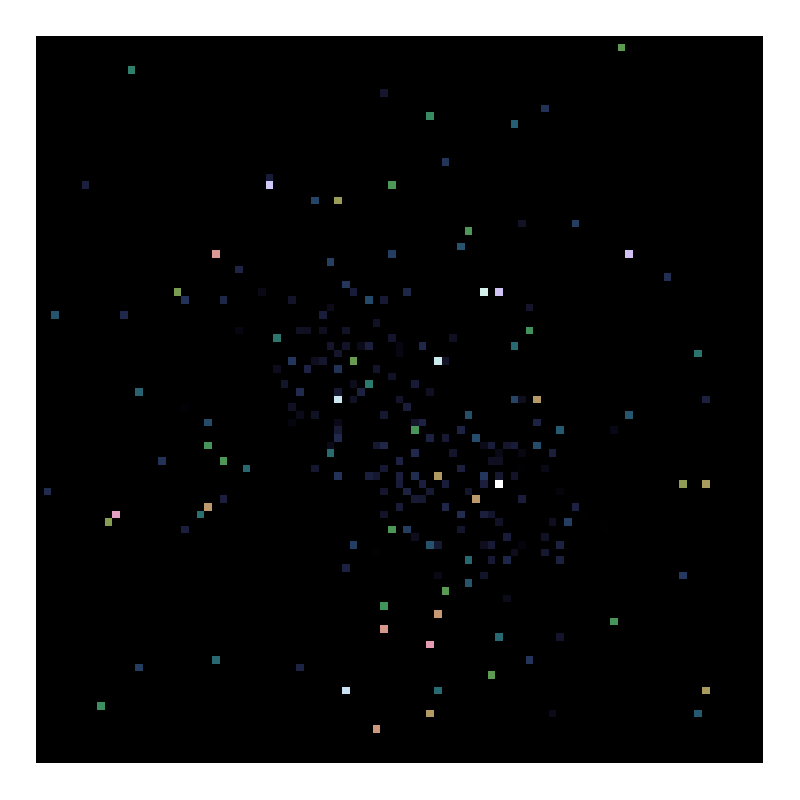
\includegraphics[width=1.00\linewidth, clip, trim= 0.25in 0.25in 0.25in 0.25in]{./chapters/05.pcdm/randomProblem/random_1k_block1.png}
		\caption{8k iterations}
		\label{pcdm:adaption:randomProblem:block11}
	\end{subfigure}
	\begin{subfigure}[b]{0.245\linewidth}
		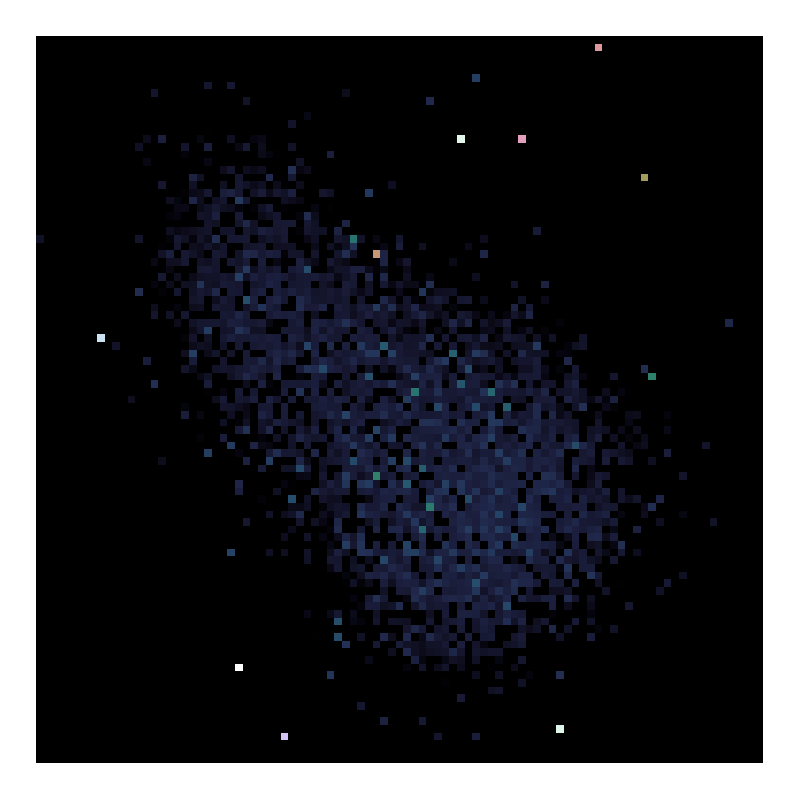
\includegraphics[width=1.00\linewidth, clip, trim= 0.25in 0.25in 0.25in 0.25in]{./chapters/05.pcdm/randomProblem/random_10k_block1.png}
		\caption{80k iterations}
		\label{pcdm:adaption:randomProblem:block12}
	\end{subfigure}
		\begin{subfigure}[b]{0.245\linewidth}
		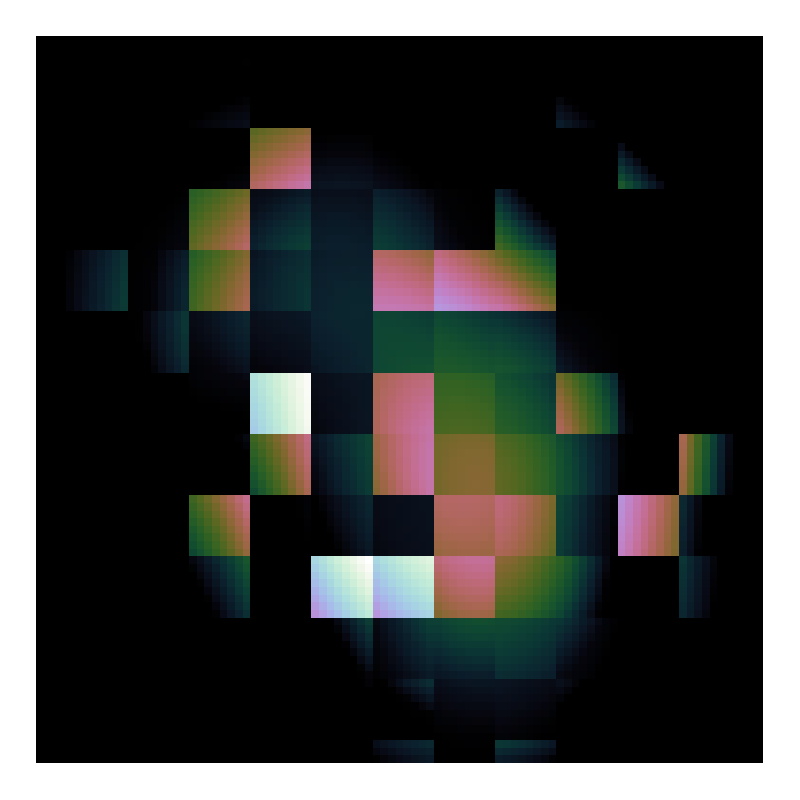
\includegraphics[width=1.00\linewidth, clip, trim= 0.25in 0.25in 0.25in 0.25in]{./chapters/05.pcdm/randomProblem/random_1k_block8.png}
		\caption{8k iterations, $8^2$ block}
		\label{pcdm:adaption:randomProblem:block81}
	\end{subfigure}
		\begin{subfigure}[b]{0.2405\linewidth}
		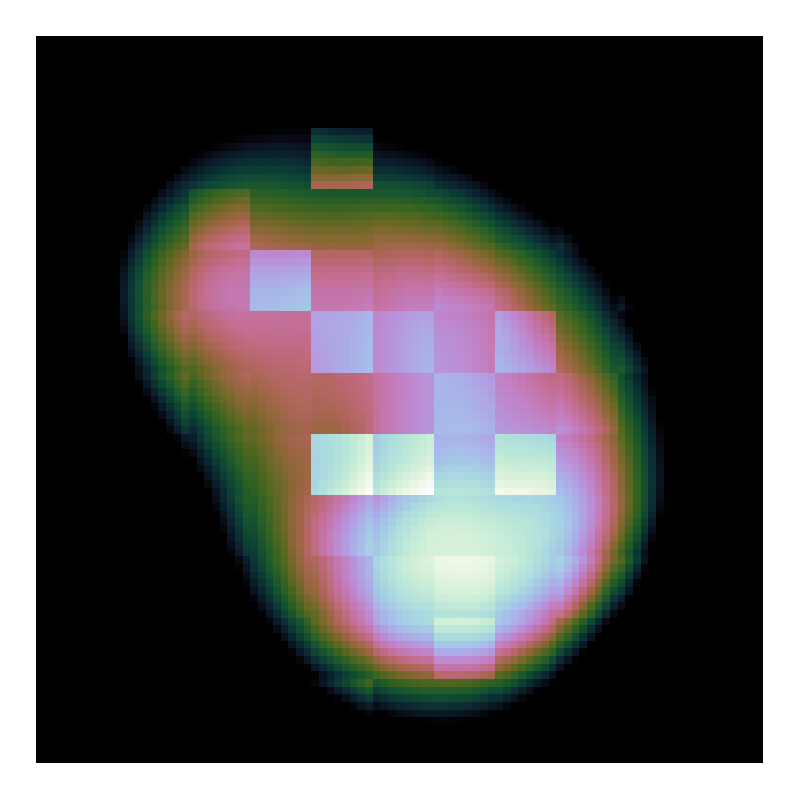
\includegraphics[width=1.00\linewidth, clip, trim= 0.25in 0.25in 0.25in 0.25in]{./chapters/05.pcdm/randomProblem/random_10k_block8.png}
		\caption{80k iterations, $8^2$ block}
		\label{pcdm:adaption:randomProblem:block82}
	\end{subfigure}
	\caption{Random parallel deconvolutions on the LMC N132D supernova remnant.}
	\label{pcdm:adaption:randomProblem}
\end{figure}

The Figure \ref{pcdm:adaption:randomProblem} shows the behavior on the LMC observation. The reconstructions receive obvious artifacts from the random selection strategy. The pixels, which get selected in the first few iterations, keep their over-estimated values. The parallel algorithm needs to select them several times to reduce their value. That is why even after 80k iterations, the N132D supernova remnant gets only hinted at in Figure \ref{pcdm:adaption:randomProblem:block12}. Until the over-estimated pixels get selected again, the algorithm cannot do useful updates in that region.

This behavior is pronounced when we choose a block size of one pixel (i.e. we do not group pixels into blocks). A naive solution is to increase the block size. This leads to fewer possible blocks in the image, and obviously an increased chance to select the same block again in later iterations. But as we see in Figure \ref{pcdm:adaption:randomProblem:block82}, the same problem exists with larger block sizes, although less pronounced. After 80k iterations the N132D supernova remnant is visible, but a few random blocks still contain too much of the emission in that area.

A random selection strategy needs a prohibitive large number of iterations to converge. But we cannot simply switch out the selection strategy. The random selection strategy is at the core of the Parallel coordinate descent methods. Remember the ESO arises from the fact that we select $tau$ pixels uniformly at random. When we select $\tau$-pixels with a greedy strategy, we might break the ESO, and the parallel algorithm may not converge at all.

To solve this behavior, we introduce the pseudo-random selection strategy:  We select a pixel at random, but greedily search in the neighborhood for the optimal pixel to optimize. The size of the neighborhood can be defined by the user as the 'Search Factor' parameter. It is essentially a mix between a greedy and a random selection strategy. If we choose a Search Factor of $1.0$, the neighborhood is the whole image, and we arrive at a greedy strategy. If we choose a Search Factor of $0.0$, then the neighborhood is one pixel, and we are back at a random strategy. The mixture of the greedy and random strategy allows us to fix the problems with the pure random strategy, without breaking any assumptions from the ESO. The optimal value for the Search Fraction is explored later in Section \ref{pcdm:results:fraction}.

We have developed three related extensions, which speed up the parallel coordinate descent algorithm in practice. We use an active set, a restarting strategy, and a 'Minor' cycle. The active set only allows the parallel algorithm to choose from a subset of pixels, which are likely to be non-zero in the final image. The restarting strategy resets the active set when it may not contain relevant pixels. Restarting is an important strategy for gradient accelerated algorithms, which have not been discussed in this section. Lastly, we re-introduce a 'Minor' cycle. The parallel coordinate descent algorithm can exploit our $PSF$ approximation scheme. With increasingly small $PSF$ windows, the parallel algorithm achieves ever faster convergence times. But the downside is it also requires more Major cycles to converge. To combat this problem, we periodically reset the residual image: We convolve the intermediate solution with the full $PSF$, and subtract it from the residuals. This is what we call a 'Minor' cycle. How these three extensions work in detail can be found in the attachments.





\section{Tests on MeerKAT LMC observation}\label{results}
The Large Magellanic Cloud (LMC) is a galaxy is the second or third closest galaxy to the Milky Way. Figure \ref{results:LMC} shows the LMC in both optical and radio wavelenghts. The radio wavelengths was observed by the VLA radio interferometer\cite{bock1999sumss} at 843MHz. In the optical wavelengths, the abundance of stars are clearly visible. The LMC is close enough to earth for individual stars are visible. But it also contains a large number of supernova remnants, gas clouds, and other extended emissions, which shine bright in the radio wavelengths.
 
The LMC is a region with a large number of sources at different brightness. In the lower-right quadrant of the radio-image \ref{results:LMC:radio}, we see the bright emission of the supernova remnant N132D, the brightest radio source in the LMC. But around the N132D are faint emissions from gas-clouds. This means faint emissions may get lost next to N132D. We need a deconvolution algorithm to uncover these faint emissions.
 
We received a MeerKAT observation of the LMC from SARAO for the purpose of algorithm testing. At the time of writing, the MeerKAT instrument is still being tested. The observation is only representative in the data volume. The observation is calibrated, and averaged down in both frequency and time. The averaging reduces both the disk space and the runtime costs of the gridding step. Nevertheless, the observation takes up over 80 GB of disk space (roughly $\frac{1}{30}$ of the original data). A CLEAN reconstruction of the calibrated observation is shown in Figure \ref{results:LMC:meerkat}.
 
\begin{figure}[h]
	\centering
	\begin{subfigure}[b]{0.3\linewidth}
		\includegraphics[width=1.0\linewidth]{./chapters/10.results/LMC/optical_cut.png}
		\caption{Optical wavelength}
	\end{subfigure}
	\begin{subfigure}[b]{0.30\linewidth}
		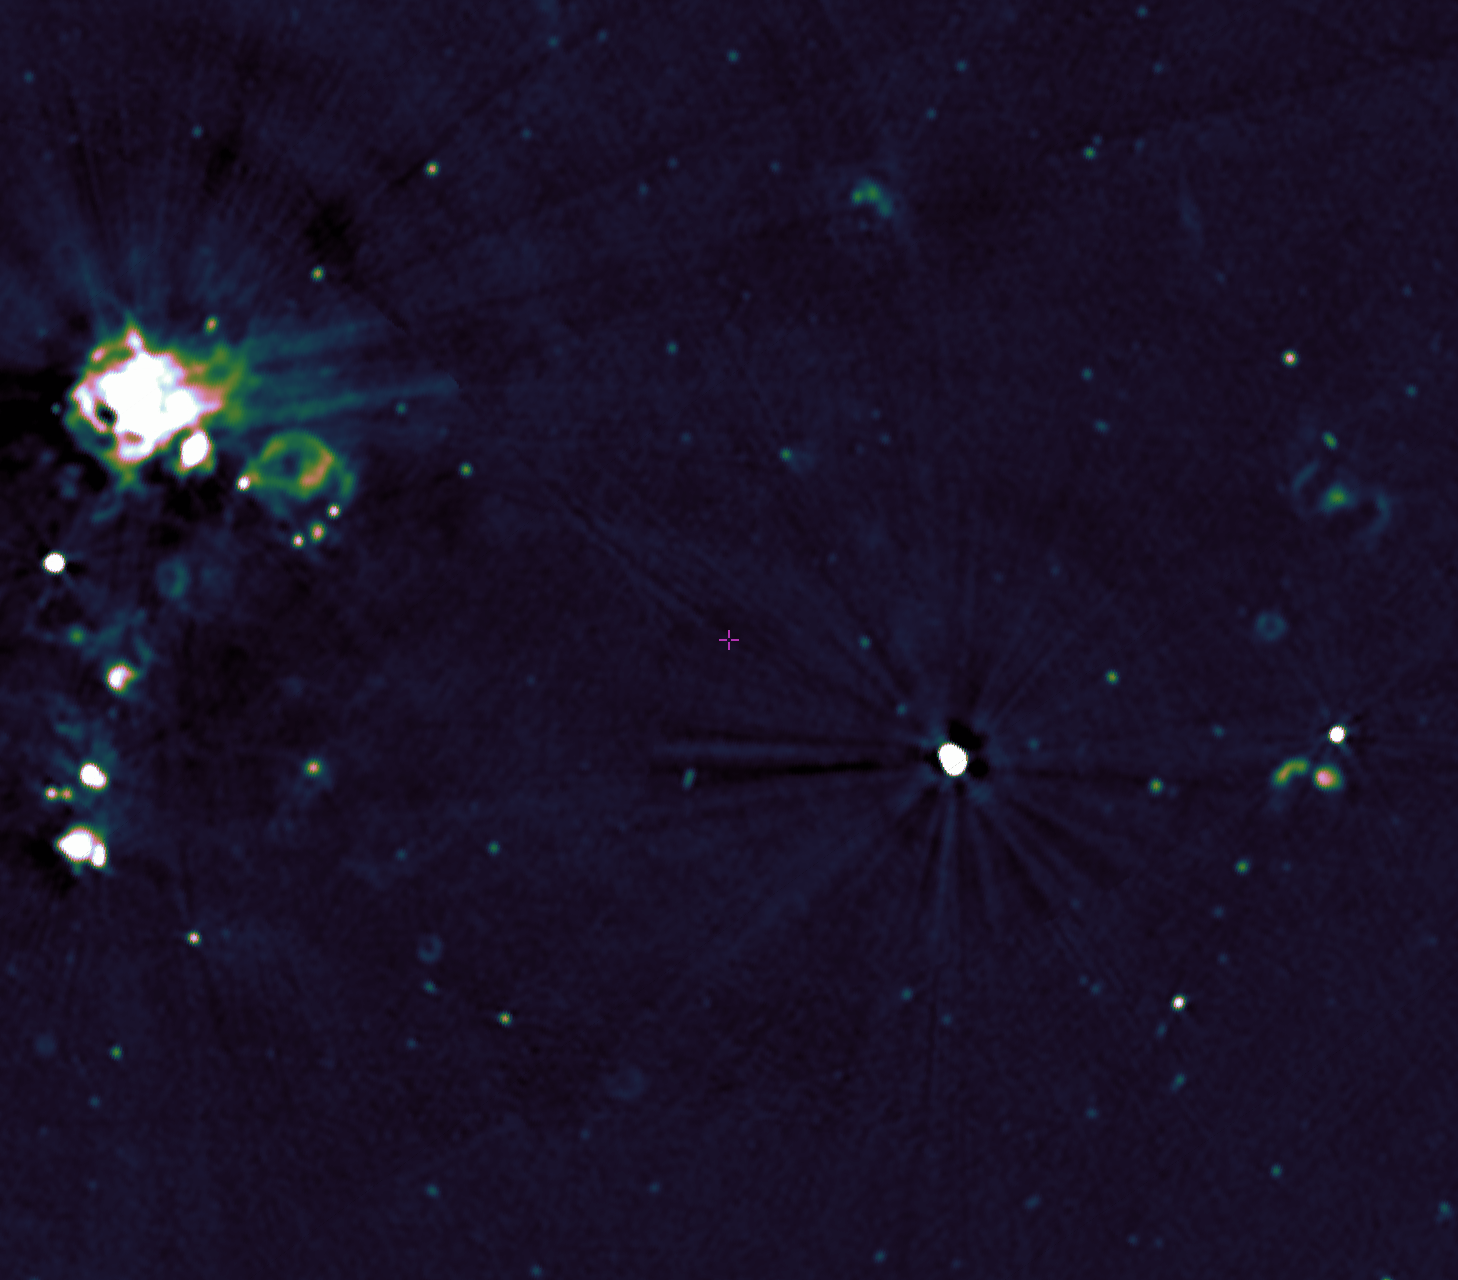
\includegraphics[width=1.0\linewidth]{./chapters/10.results/LMC/radio-843_cut.png}
		\caption{Radio wavelength at 843MHz.}
		\label{results:LMC:radio}
	\end{subfigure}
	\begin{subfigure}[b]{0.375\linewidth}
		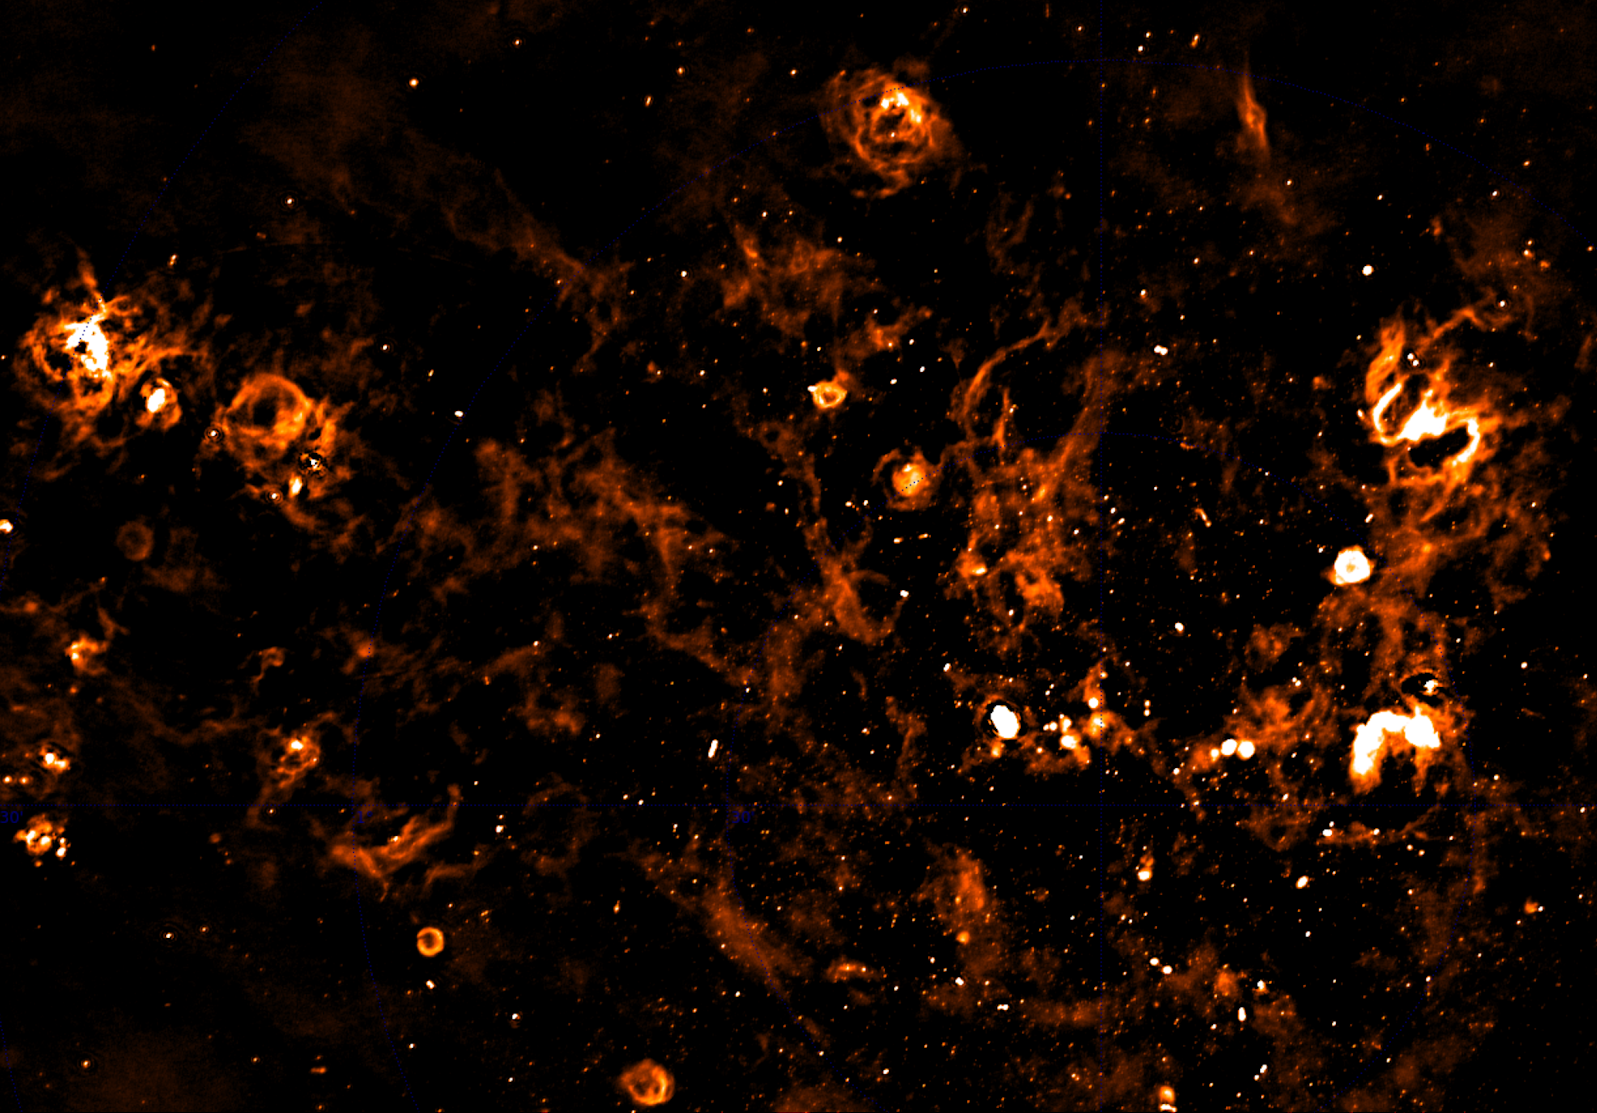
\includegraphics[width=1.0\linewidth]{./chapters/10.results/LMC/meerkat2.png}
		\caption{Wide band radio image by MeerKAT.}
		\label{results:LMC:meerkat}
	\end{subfigure}
	\caption{Section of the Large Magellanic Cloud (LMC)}
	\label{results:LMC}
\end{figure}

The MeerKAT observation covers a wide band of radio frequencies. The lowest frequency in the MeerKAT observation is 894 MHz, and the highest frequency is
Imaging the whole frequency band requires a wide band deconvolution algorithm. In wide band imaging, several images at different frequencies get deconvolved as an image cube. Wide band imaging again multiplies the amount of work that has to be done for reconstruction, as now we cannot deconvolve a single image, but have to deal with a whole image cube.

Wide band imaging is not possible within the time frame of this project. We take a narrow band subset of 5 channels from the original data (ranging from 1084 to 1088 MHz, about 1 Gb in size) for reconstruction. We also reduce the field-of-view to a more manageable section. Figure \ref{results:cutout} shows the LMC image section we are using together with a CLEAN reconstruction of the narrow band data.

\begin{figure}[h]
	\centering
	\begin{subfigure}[b]{0.4\linewidth}
		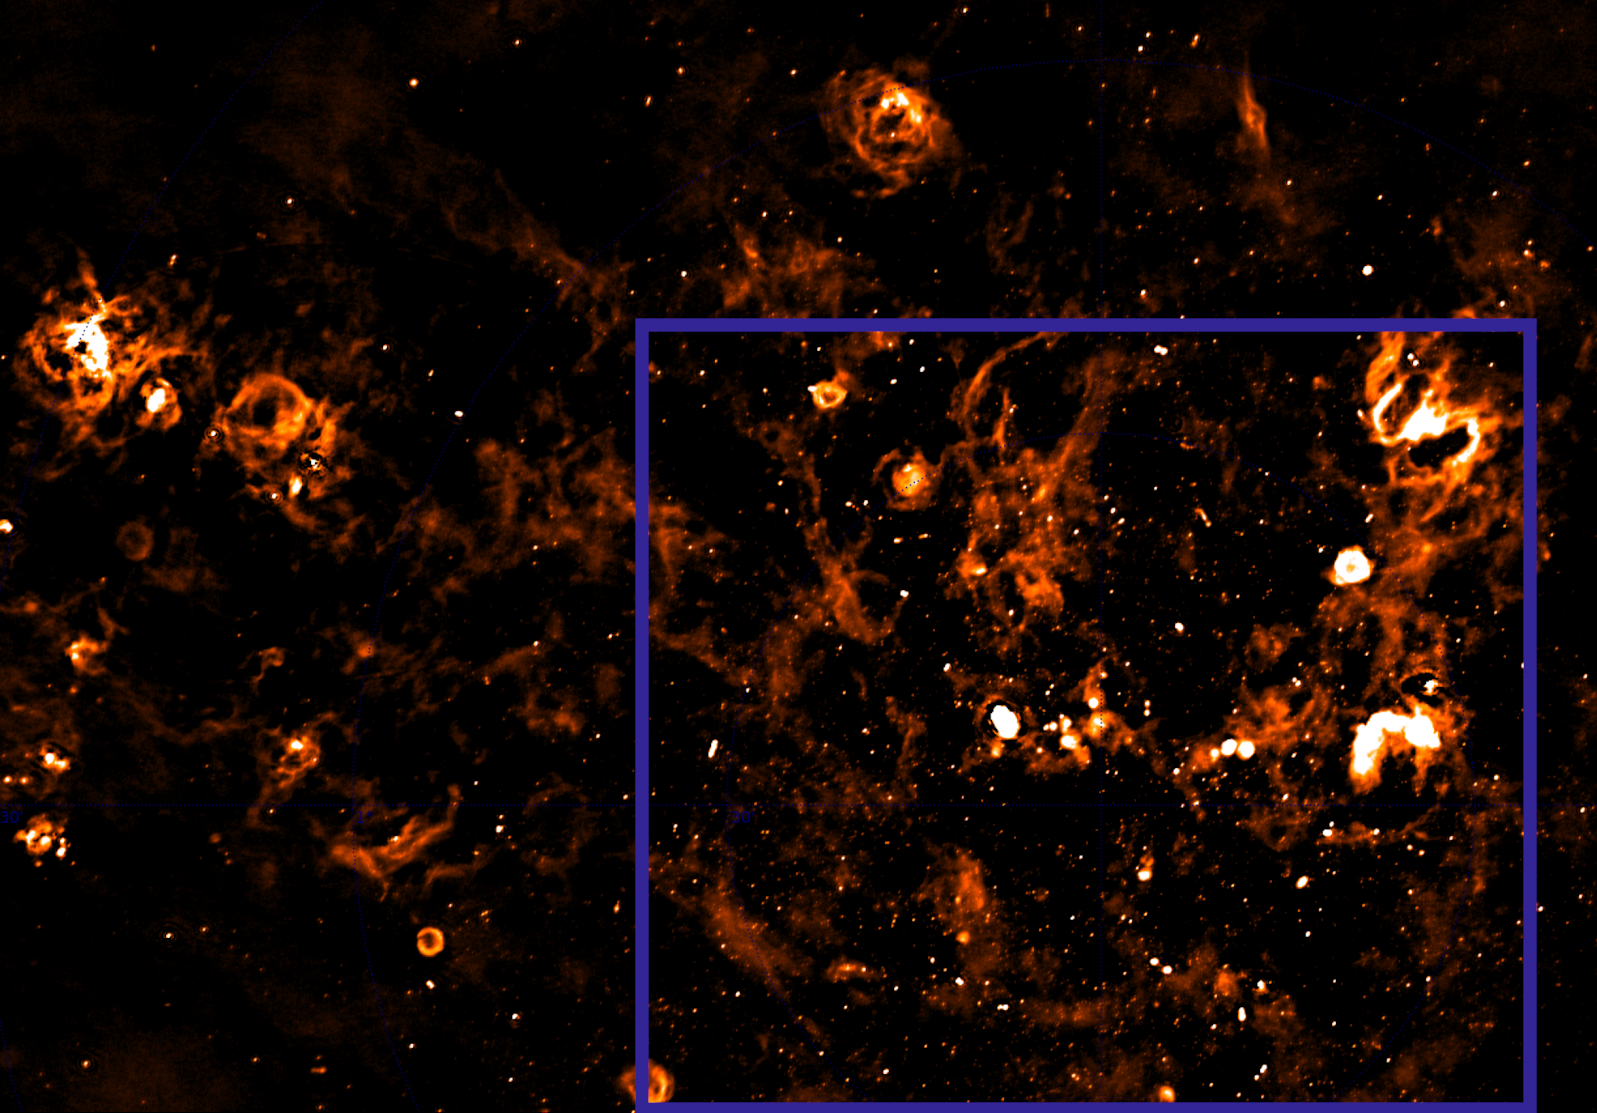
\includegraphics[width=1.0\linewidth]{./chapters/10.results/LMC/meerkat_cutout.png}
	\end{subfigure}
	\begin{subfigure}[b]{0.30\linewidth}
		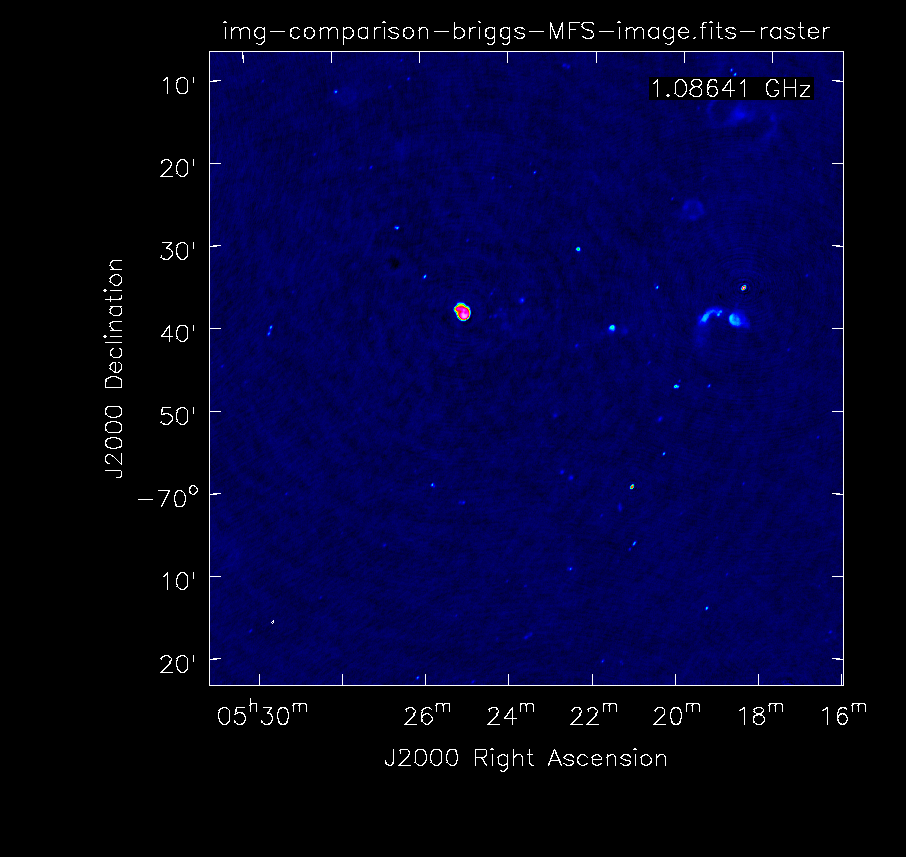
\includegraphics[width=1.0\linewidth]{./chapters/10.results/cleancomp/clean_briggs.png}
	\end{subfigure}
	\caption{Narrow band image section used.}
	\label{results:cutout}
\end{figure}

At the center of our image section \ref{results:cutout} we see the N132D supernova remnant. We partially see the faint extended emissions, although they are close to the noise level. This is known as a high-dynamic range reconstruction. We have strong radio sources mixed together with faint emissions, which are only marginally above the noise level of the image.

The total field-of-view of our image section is roughly 1.3 degrees(or 4600 arc seconds). Our reconstruction has $3072^2$ pixel with a resolution of 1.5 arc seconds per pixel. this is still a wide field-of-view reconstruction problem. We have to account for the effects of the $w$-term to achieve a high-dynamic range reconstruction.

In our test reconstruction, we need to account for $w$-term correction and high-dynamic range. We have excluded wide-band imaging as not feasible within the time frame of this project. In Section \ref{results:cleancomp} we compare the reconstructions of CLEAN with our coordinate descent based algorithm on the LMC observation. The next Section \ref{results:speedup} presents the speedup we achieve with coordinate descent by using our distributed or GPU-accelerated implementations.

In Section \ref{results:gradients} we show the core result of this project. Namely what effect has an approximate $PSF$ on the deconvolution problem and whether we can use it to further distribute the problem. The answer to that question is affirmative: We can approximate the $PSF$, and we can exploit it to further distribute the deconvolution. But we need more sophisticated coordinate descent algorithms to fully benefit from it.


\subsection{Comparison with CLEAN reconstructions} \label{results:cleancomp}
We use the WSCLEAN \cite{offringa2014wsclean} implementation of multi-scale CLEAN. We compare our coordinate descent reconstruction with two CLEAN reconstructions, oe with naturally weighted visibilities and one with briggs weighted visibilities.

There are three main visibility weighting scheme for the gridder that lead to different $PSF$s from the same measurements: Natural, uniform, and Briggs\cite{briggsWeighting}. Natural weighting scheme leads to an image with a lower noise level, but a wider $PSF$. Uniform weighting leads to a higher noise level, but to a $PSF$ whgich is more concentrated around a single pixel. Briggs weighting is a scheme combines the best from both worlds, receiving an image with acceptable noise level while getting a more concentrated $PSF$. As such it is widely used in radio astronomy image reconstruction. Our gridder implements the natural weighting scheme only. Nevertheless our coordinate descent algorithm is able to retrieve structures similar to the briggs-weighted multi-scale CLEAN reconstruction, even though coordinate descent has to work with a wider $PSF$.

\begin{figure}[h]
	\centering
	\begin{subfigure}[b]{0.4\linewidth}
		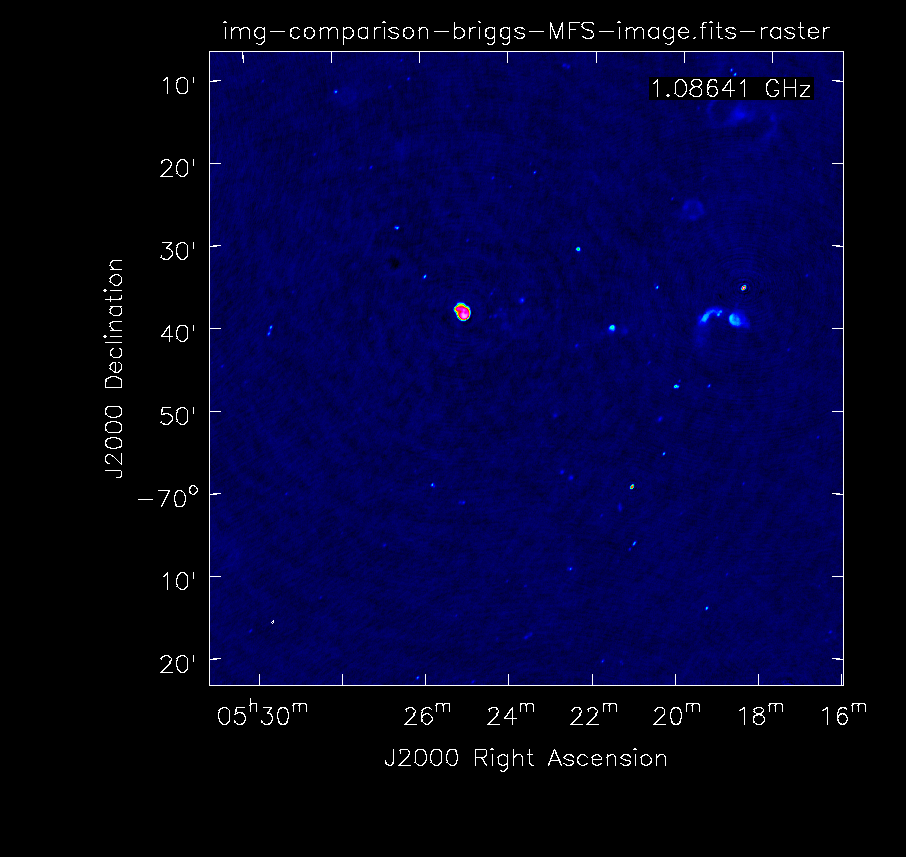
\includegraphics[width=1.00\linewidth]{./chapters/10.results/cleancomp/clean_briggs.png}
		\caption{Briggs weighted multi-scale CLEAN.}
		\label{results:comp:clean}
	\end{subfigure}
	\begin{subfigure}[b]{0.40\linewidth}
		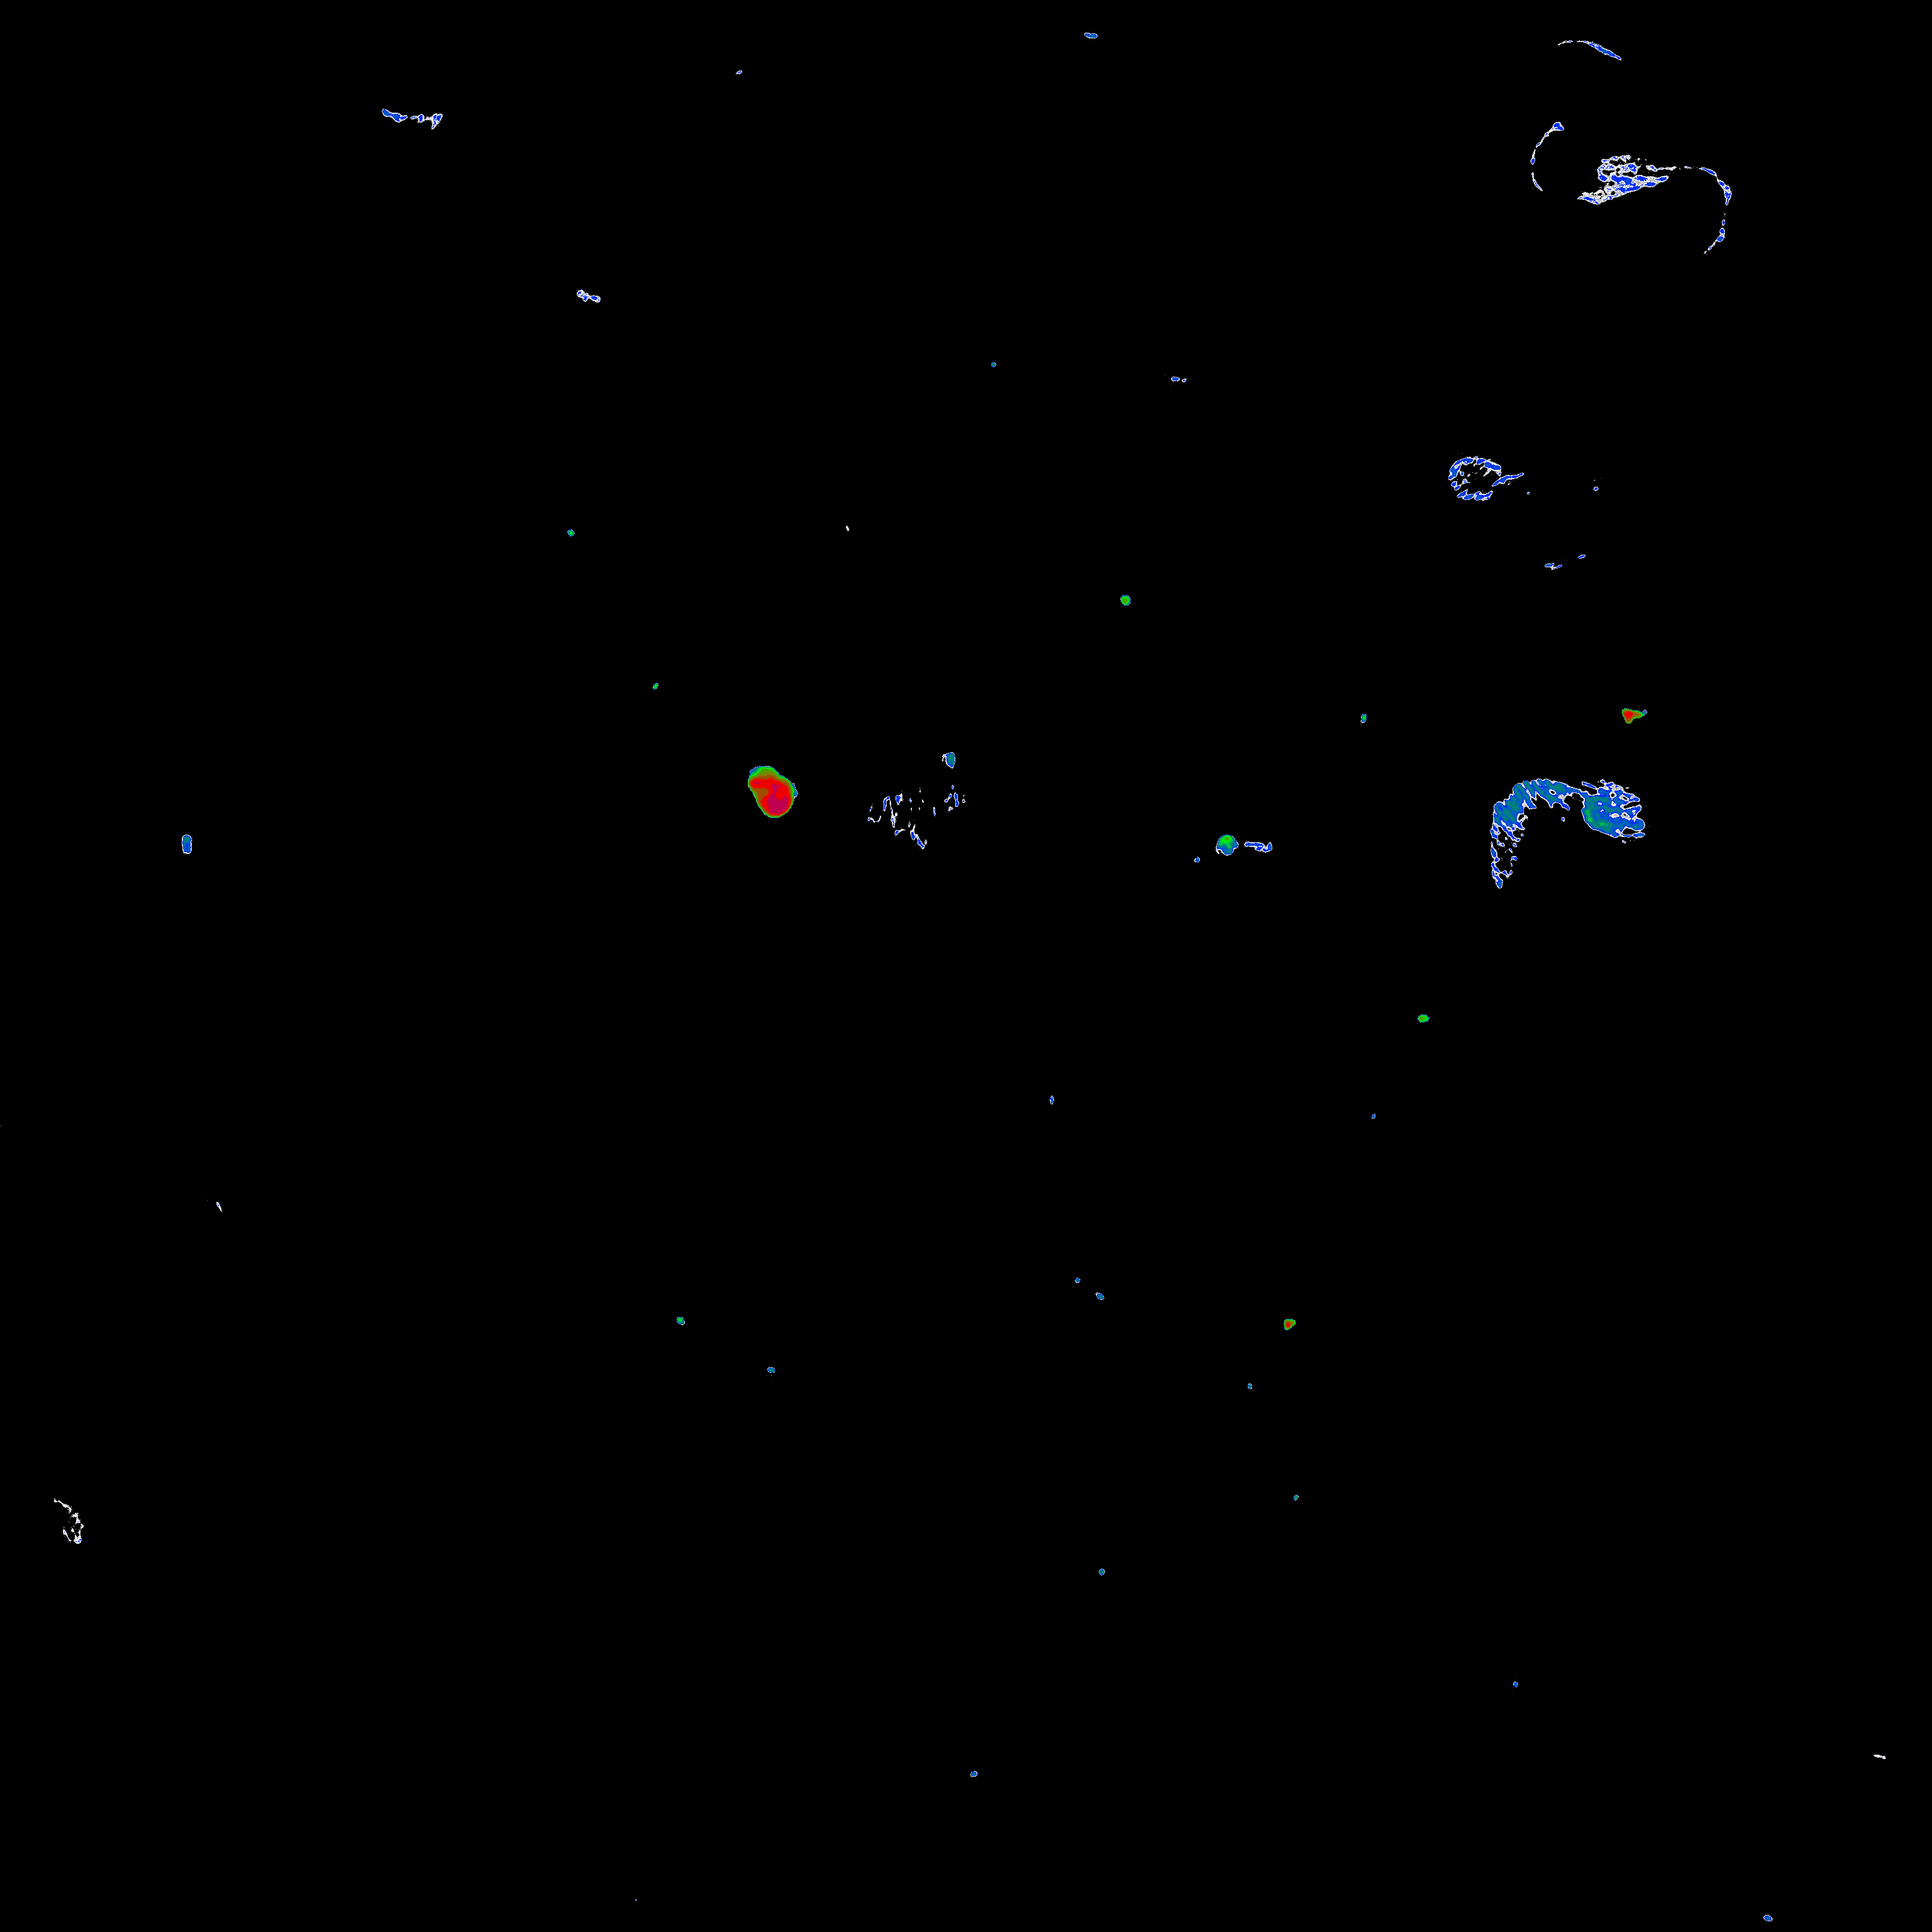
\includegraphics[width=1.00\linewidth]{./chapters/10.results/cleancomp/cd.png}
		\caption{Naturally weighted coordinate descent.}
		\label{results:comp:cd}
	\end{subfigure}
	\caption{Comparison of the whole image}
	\label{results:cleancomp:figure}
\end{figure}

Figure \ref{results:cleancomp:figure} shows the reconstruction of both briggs-weighted multi-scale CLEAN and the naturally weighted coordinate descent reconstruction.
%parameters for CLEAN and Coordinate descent. Lambda and alpha
CLEAN used 6 major cycles and 14 thousand minor cycle iterations. Our coordinate descent implementation converged after 5 major cycles and needed 100 thousand iterations to converge.

Coordinate descent needs a large number of iterations to converge when compared to multi-scale CLEAN. Note that a coordinate descent iteration is cheaper to compute than one iteration of multi-scale CLEAN. Also note that because we are searching for structures close to the noise level of the image, coordinate descent often adds pixels belonging to the noise in one major cycle, just to remove them in the next one. Path regularization\cite{friedman2010regularization} can combat this problem, and gets further investigated in the following Section \ref{results:gradients}.

Both algorithms detect the three extended emissions at the right side of the image. They detect various point sources at the same location. Coordinate descent and multi-scale CLEAN arrive at a roughly similar result. Coordinate descent detects similar structures in the N132 supernova remnant, as the briggs-weighted CLEAN, but also includes calibration errors in its reconstruction of the faint extended emissions.

\begin{figure}[h]
	\centering
	\begin{subfigure}[b]{0.3\linewidth}
		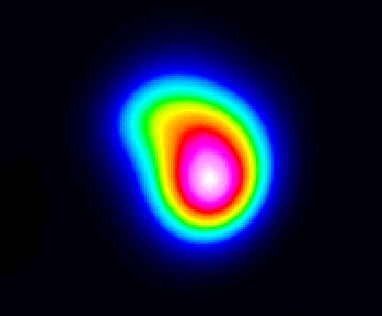
\includegraphics[width=1.00\linewidth]{./chapters/10.results/cleancomp/n132_clean.png}
		\caption{CLEAN Natural weighting.}
		\label{results:N132:clean}
	\end{subfigure}
	\begin{subfigure}[b]{0.3\linewidth}
		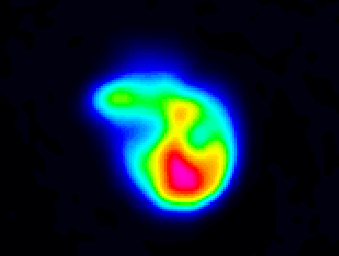
\includegraphics[width=1.00\linewidth]{./chapters/10.results/cleancomp/n132_clean_briggs.png}
		\caption{CLEAN Briggs weighting.}
		\label{results:N132:cleanbriggs}
	\end{subfigure}
	\begin{subfigure}[b]{0.3\linewidth}
		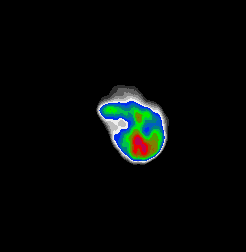
\includegraphics[width=1.00\linewidth]{./chapters/10.results/cleancomp/n132_cd.png}
		\caption{CD Natural weighting.}
		\label{results:comp:N132:cd}
	\end{subfigure}
	\caption{N132 comparison}
	\label{results:cleancomp::N132:figure}
\end{figure}

Figure \ref{results:cleancomp::N132:figure} compares the naturally-weighted CLEAN, briggs CLEAN and coordinate descent on the N132 supernova remnant. The naturally-weigted CLEAN and coordinate descent use the same $PSF$ for the deconvolution. But coordinate descent finds structures in N132 similar to the briggs-weighted CLEAN. Coordinate descent arrived at a plausible higher-resolved reconstruction of N132.

\begin{figure}[h]
	\centering
	\begin{subfigure}[b]{0.3\linewidth}
		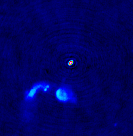
\includegraphics[width=1.00\linewidth]{./chapters/10.results/cleancomp/clean_calibration.png}
		\caption{Briggs CLEAN}
	\end{subfigure}
	\begin{subfigure}[b]{0.3\linewidth}
		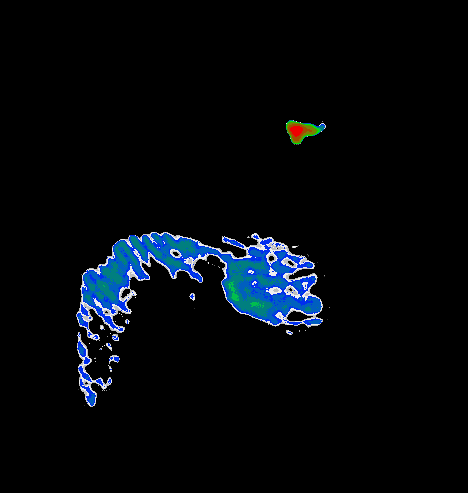
\includegraphics[width=1.00\linewidth]{./chapters/10.results/cleancomp/cd_calibration.png}
		\caption{Coordinate Descent}
	\end{subfigure}
	\caption{Influence of calibration errors}
	\label{results:cleancomp::calib:figure}
\end{figure}

Calibration errors on the other hand negatively influence the coordinate descent reconstruction. Figure \ref{results:cleancomp::calib:figure} shows a cutout of the right hand section of the reconstruction, where a faint extended emission is next to a point source with calibration errors. Multi-scale CLEAN is able to differentiate between the "ripples" from the calibration error, and the signal from the extended emission. Coordinate descent with the elastic net regularization includes the ripples into the reconstructed image. 

The only way to exclude the ripples from the reconstruction is to increase the regularization parameter $\lambda$., such as no pixel gets included which is not above the noise level + calibration error in the image. However, that would lead to other sources being "regularized away" in other regions of the image, which do not have a severe calibration error close by. 


Case of super resolution.
Our coordinate descent algorithm works. All the performance optimizations do not break anything vital.


\subsection{Coordinate descent acceleration with MPI or GPU}\label{results:speedup}
Describe hardware

Distributed with MPI

GPU implementation

Measurement of the speedup.

\begin{figure}[h]
	\centering
		\begin{subfigure}[b]{0.4\linewidth}
		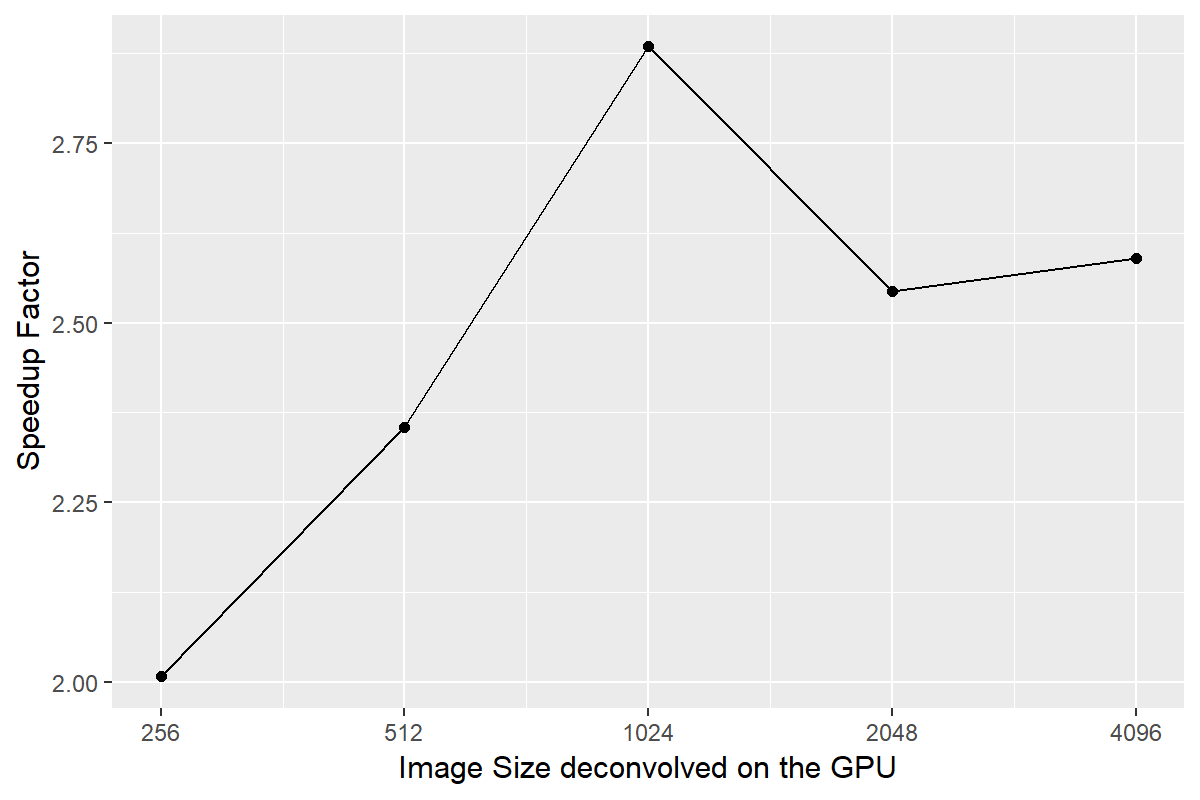
\includegraphics[width=1.00\linewidth]{./chapters/10.results/speedup/gpu.png}
	\end{subfigure}
	\begin{subfigure}[b]{0.4\linewidth}
		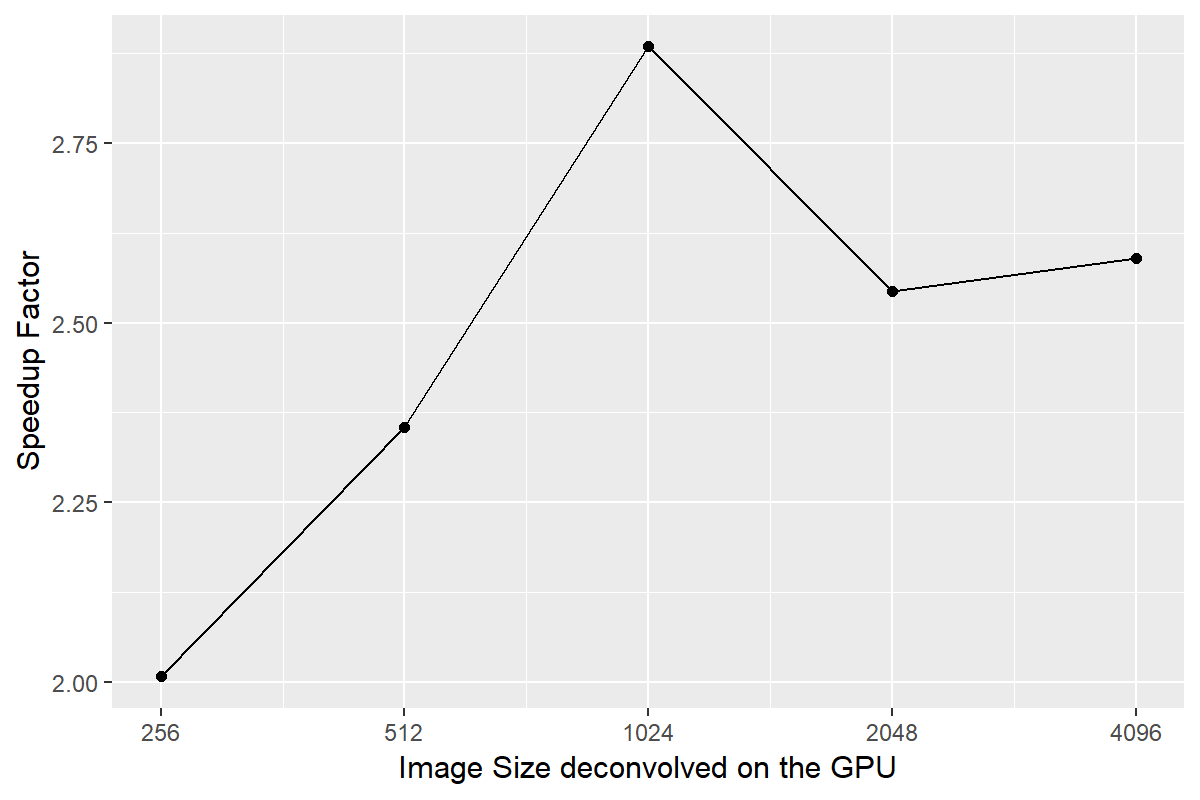
\includegraphics[width=1.00\linewidth]{./chapters/10.results/speedup/gpu.png}
	\end{subfigure}
	\caption{Speedup by using MPI or GPU acceleration}
	\label{results:speedup:figure}
\end{figure}


We cannot use MPI combined with the GPU. The MPI implementation uses a communication step in each coordinate descent iteration (communicating which pixel to optimize with MPI Allreduce). 



\subsection{Effect of approximating the $PSF$} \label{results:gradients}
As we described in Section \ref{gradients}, the $PSF$ for deconvolution is as big as the image. For wide field-of-view observations of MeerKAT, the $PSF$ is approximately a gaussian with decreasing pixel values the further we move from the center. Most of the values in the $PSF$ are close to zero. The question is, what effect has an approximate deconvolution with a smaller $PSF$? If we can approximate the deconvolution with a small enough $PSF$, we can solve patches of the image independently of each other. However, the $PSF$ approximation may need more major cycles to converge.

The effect of approximating the $PSF$ are not clear. We know that thanks to the $w$-term in the visibilities, the $PSF$ is not constant over the image. We already need several major cycles to converge. With a good approximation of the $PSF$, we may speed up the individual iterations of coordinate descent without needing more major cycle.

We presented two methods to approximating the $PSF$ for the deconvolution in Section \ref{gradients}. Method 1 updates only a fraction of the gradients, and Method 2 uses a fraction of the $PSF$ for deconvolution. We test both methods on the LMC data and explore what effects the approximations have on the reconstruction.

\subsubsection{Method 1: Approximate gradient update}
Our coordinate descent method updates the map of gradients after each iteration. This method only updates the most significant fraction of the gradients.
Method 1 starts with the same map of gradients as the original, but then only updates a fraction of the gradients in each iteration. It updates a rectangle of the most significant gradients.
With each iteration, the map of gradients gets less accurate. With enough major cycles, this method converges to the same optimum as the original coordinate descent method.

At the beginning of each major cycle, we calculate the objective value of the current solution. We compare the objective value and the wall-clock time of the original and the approximate gradient update. 
Target: get the lowest possible objective value.
Figure \ref{results:gradients:update} shows the results.

\begin{figure}[h]
	\centering
	\begin{subfigure}[b]{0.7\linewidth}
		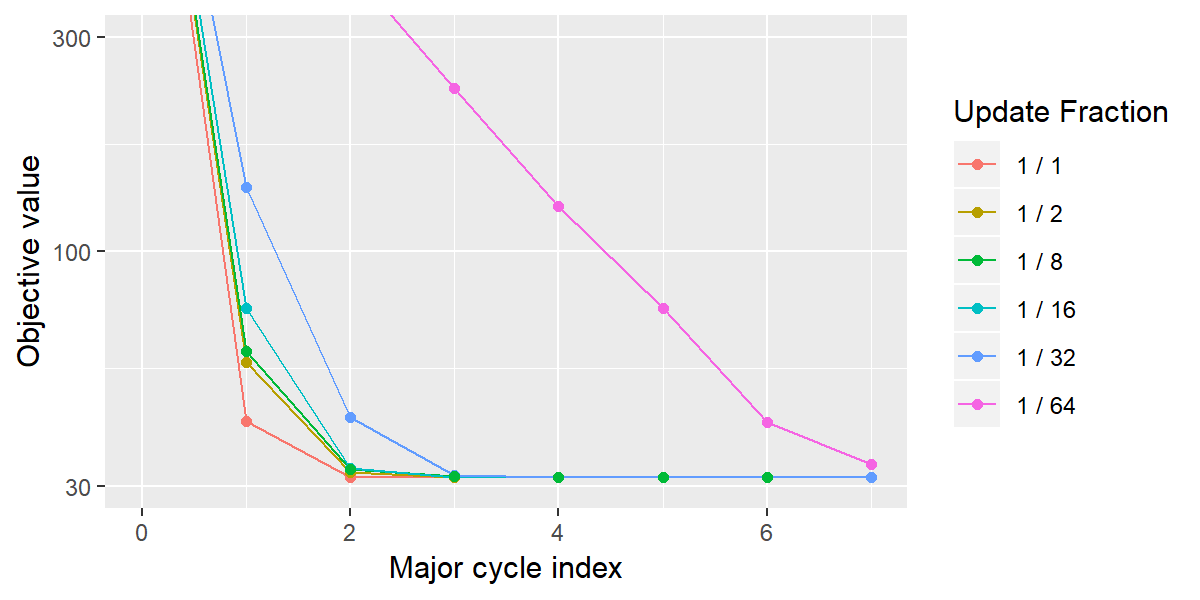
\includegraphics[width=\linewidth]{./chapters/10.results/gradient/ApproxUpdate/size.png}
	\end{subfigure}
	\\
	\begin{subfigure}[b]{0.35\linewidth}
		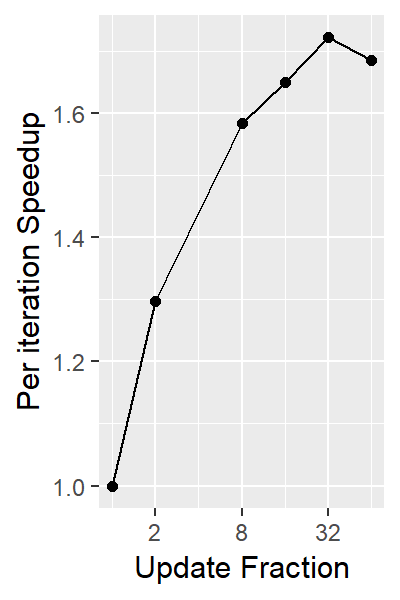
\includegraphics[width=\linewidth]{./chapters/10.results/gradient/ApproxUpdate/speedup_iter.png}
	\end{subfigure}
	\begin{subfigure}[b]{0.35\linewidth}
		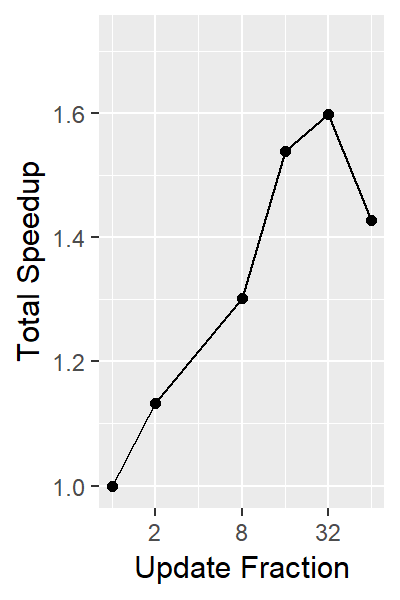
\includegraphics[width=\linewidth]{./chapters/10.results/gradient/ApproxUpdate/speedup_total.png}
	\end{subfigure}
	
	\caption{Effect of only updating a fraction of the gradients.}
	\label{results:gradients:update}
\end{figure}

The smallest possible fraction in which our solution still converges is $\frac{1}{64}$. This updates only the $48^2$ most siginificant gradients.

We seem to converge. Objective value of the approximations is within 0.03\% of the original (the objective value of the approximations are higher by a factor of 0.0003).
We cannot report an error that correlates with the fraction of the update. The objective value of $\frac{1}{2}$ is above the value of $\frac{1}{32}$.

The speedup is harder to quantify. For one, each iteration gets cheaper. For another, the number of iterations also change. We measured both, the speedup for one coordinate descent iteration, and the total speedup.

Implicit path regularization. Coordinate descent profits from an ever decreasing $\lambda$. This is done implicitly for the approximation of gradient updates. We have to stop before we include bad things.

Major cycles.

Overall, no. We can 

\subsubsection{Method 2: Approximate deconvolution}
In this method, we use a fraction of the total $PSF$ for deconvolution. This method solves a different deconvolution problem, where the $PSF$ is for example only $\frac{1}{8}$ the size. The downside is that method 2 is not guaranteed to converge to the same optimum. Nevertheless, we solve the approximate deconvolution problem with several different fractions of the $PSF$ and compare how close the approximate solution is to the original.

We measure the true objective value for the approximate solution at the beginning of each major cycle iteration. The Figure \ref{results:gradients:aproxDeconv} compares the approximate deconvolutions to the deconvolution with the full $PSF$

\begin{figure}[h]
	\centering
	\begin{subfigure}[b]{0.7\linewidth}
		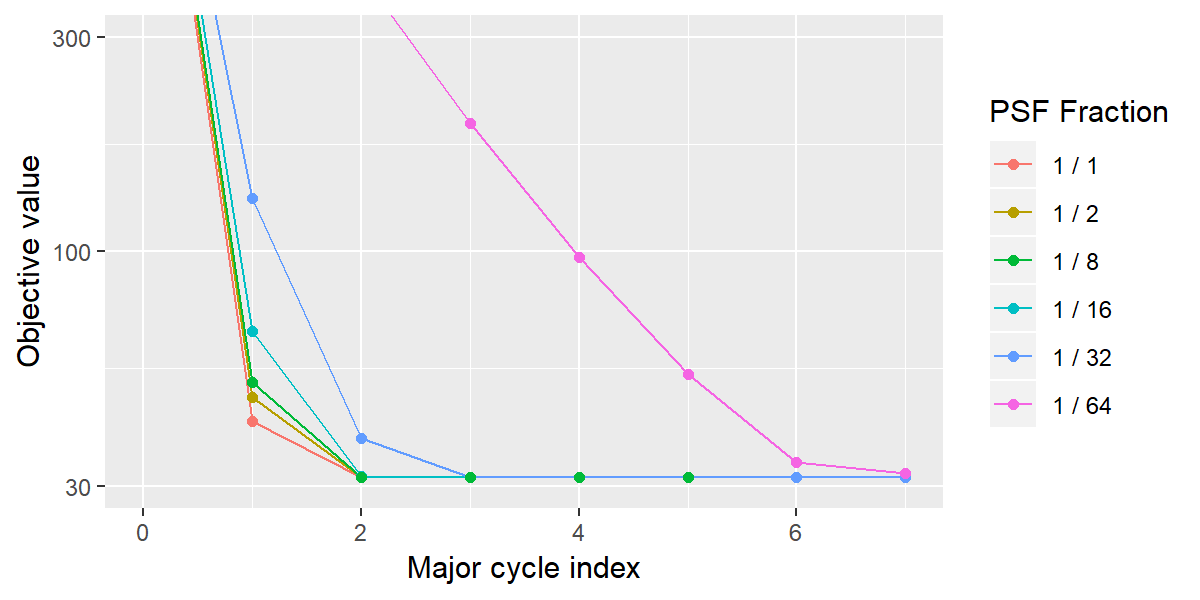
\includegraphics[width=\linewidth]{./chapters/10.results/gradient/ApproxDeconv/size.png}
	\end{subfigure}
	\\
	\begin{subfigure}[b]{0.35\linewidth}
		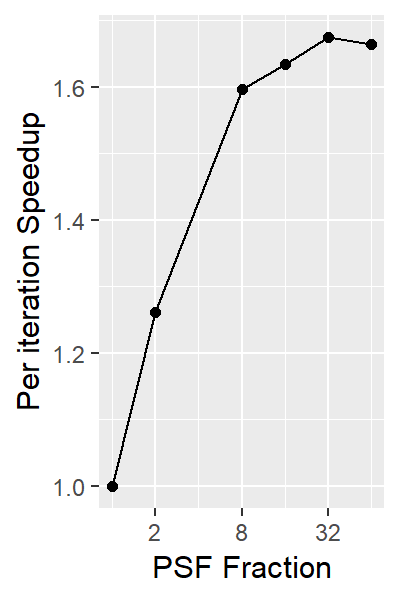
\includegraphics[width=\linewidth]{./chapters/10.results/gradient/ApproxDeconv/speedup_iter.png}
	\end{subfigure}
	\begin{subfigure}[b]{0.35\linewidth}
		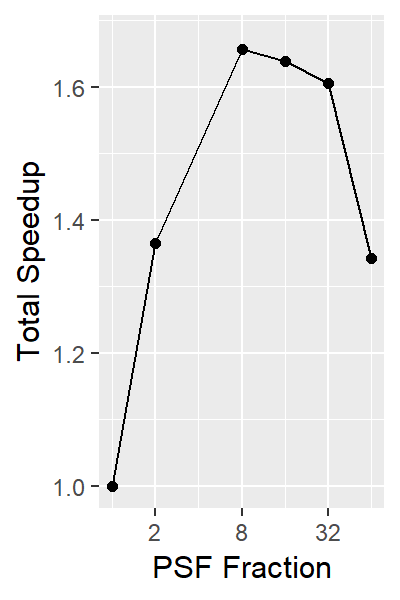
\includegraphics[width=\linewidth]{./chapters/10.results/gradient/ApproxDeconv/speedup_total.png}
	\end{subfigure}
	
	\caption{Effect of the L1 and L2 Norm separately.}
	\label{results:gradients:aproxDeconv}
\end{figure}

With $48^2$ pixels, the approximate deconvolution converges. But it is not the same optimum. The difference becomes less extreme as soon as we increase the $PSF$ size. With a factor of 32, we converge within
of the true solution. But we need a major cycle more to converge.




Just by cutting the $PSF$ coordinate descent gets a speedup. 


Approximate deconvolution

$PSF$ is the size of the image, i.e. $3072^2$ pixels. We approximate the deconvolution by just using a fraction of the $PSF$. $\frac{1}{8}$ is the size of $384^2$
We measured the objective value at the beginning of each major cycle.
Figure \ref{results:gradients:aproxDeconv} shows the decrease in objective value
and the speedup associated with cutting the $PSF$

We have an obvious limit where cutting the $PSF$ will be useless, because it does not converge.
But there is a less obvious failure mode. The $PSF$ of the size $\frac{1}{64}$ already does not properly converge, and the objective actually becomes after 3 major cycles.

We have two speedup factors. Speedup by iterations becoming cheaper, and the total time spent doing deconvolution.
Path regularization and potentially more
Path regularization and how much time we spent in the deconvolution.

One problem: we do not converge to the same optimum.

\subsubsection{Comparison Method 1 and 2}
\begin{figure}[h]
	\centering
	\begin{subfigure}[b]{1.0\linewidth}
		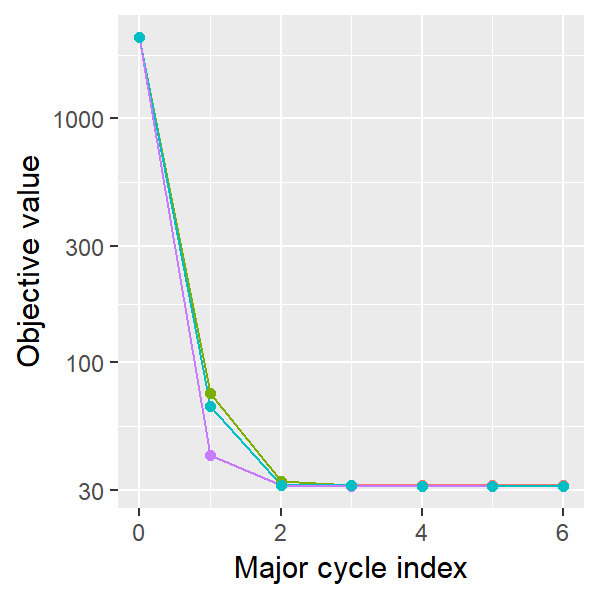
\includegraphics[width=\linewidth]{./chapters/10.results/gradient/comparison.png}
	\end{subfigure}
	\begin{subfigure}[b]{1.0\linewidth}
		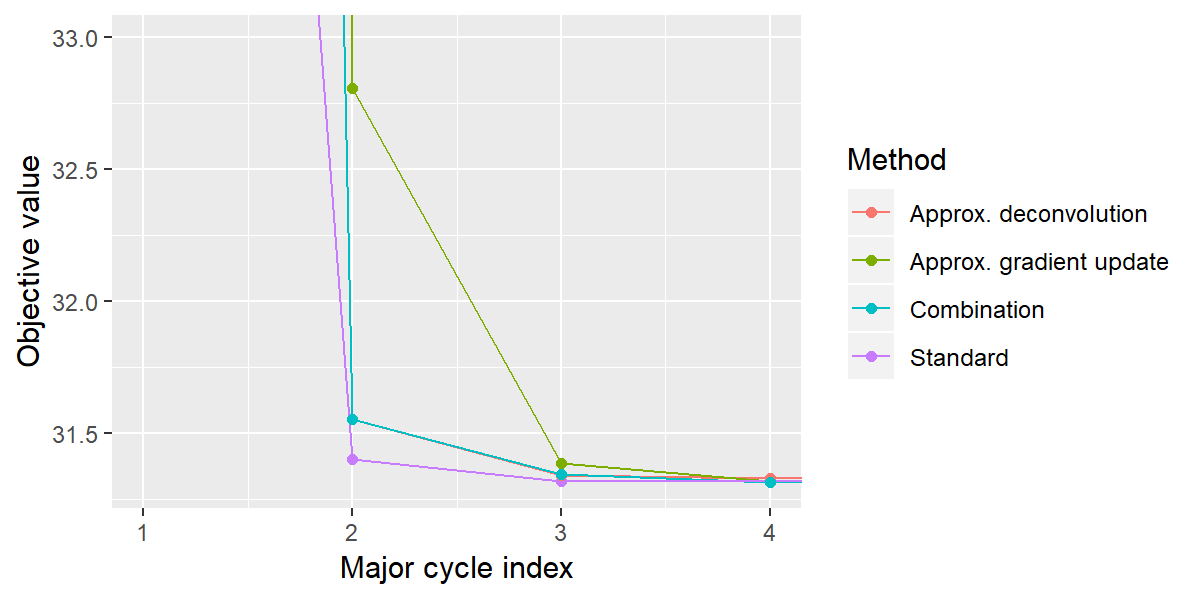
\includegraphics[width=\linewidth]{./chapters/10.results/gradient/comparison_zoom.png}
	\end{subfigure}
	
	\caption{Effect of the L1 and L2 Norm separately.}
	\label{results:gradients:comparison}
\end{figure}

\subsubsection{Masking the $PSF$}

\section{Conclusion}
In this project, we developed our own image reconstruction pipeline in .Net Core. We implemented the Image Domain Gridder\cite{veenboer2017image} and developed two deconvolution algorithms: A serial and a parallel coordinate descent deconvolution algorithm in the Major/Minor cycle architecture. 

For this project, we developed the hypothesis that a deconvolution algorithm in the Major/Minor cycle architecture may be speed up by using an approximate $PSF$. The deconvolution algorithm already uses an approximation of the true $PSF$. We showed that the $PSF$ can be further approximated, which simplifies the deconvolution problem for parallel and distributed computing. In this project, we created a novel $PSF$ approximation scheme for the Major/Minor cycle architecture, and implemented a parallel coordinate descent algorithm which can exploit the approximated  $PSF$ for a significant speedup. On our test, the parallel coordinate descent algorithm is estimated to outperform standard CLEAN in convergence speed.

The parallel coordinate descent algorithm can use modern non-blocking instructions, running in parallel deconvolutions with little communication overhead. Our implementation is optimized for the CPU on a shared-memory system. The algorithm can easily be extended for the distributed setting, where different machines deconvolve the image in parallel. The parallel coordinate descent algorithm showed competitive convergence speeds in comparison to CLEAN on the CPU. These results may be further improved by using GPU acceleration for the parallel algorithm.

The degree of parallelism scales with the problem size for the parallel coordinate descent algorithm. Large deconvolution problems can be efficiently solved by adding additional processors. This algorithm has the potential to scale with the planned expansion of MeerKAT to SKA-Mid. However, the imaging problem will also change together with MeerKAT's expansion. It remains to be seen if the parallel coordinate descent algorithm is competitive on the SKA-Mid imaging task.

We tested our $PSF$ approximation scheme and parallel coordinate descent algorithm on a real-world observation of MeerKAT. The approximation scheme and parallel algorithm are not inherently limited to a single instrument. However, our $PSF$ approximation scheme tends to be more effective on medium- to high-frequency observations. The $PSF$s of low-frequency observations cannot be approximated as efficiently. In turn, the parallel coordinate descent algorithm may not achieve the same speedups on low-frequency observations.

%The $PSF$ approximation scheme does not speed up any algorithm. For the serial coordinate descent algorithm, the $PSF$ approximation did result in speedup, but not enough to compete with CLEAN on convergence speed. One needs specialized reconstruction algorithms to exploit the $PSF$ approximation we developed in this project. The parallel coordinate descent algorithm can exploit the approximate $PSF$ for a significant speedup.

We used the elastic net regularization. To our knowledge, it is not widely used in the radio astronomy community. On our test, the elastic net regularization created more plausible reconstructions of radio sources than multi-scale CLEAN. The elastic net was also more sensitive to calibration errors in the image. This is a similar behavior to over-complete regularizations, which are often used for radio interferometric image reconstructions. However, elastic net is a significantly simpler regularization. Leading to a simpler reconstruction algorithm in a parallel or distributed setting. 

We demonstrated with the parallel coordinate descent algorithm that an elastic net regularized image can be reconstructed efficiently. These results suggests the elastic net regularization may be a viable alternative for radio interferometric image reconstruction. We tested the elastic net regularization on a single real-world observation. The question, whether elastic net is a viable alternative for image reconstruction, has to explored on multiple observations in the future.

We limited this project to the narrow-band image reconstruction only. This is the main limitation of this work. Wide-band imaging introduces new challenges for an image reconstruction algorithm. However, the parallel coordinate descent algorithm also has the potential to benefit from it. We may increase the degree of parallelism further in the wide-band imaging case. It is unknown how our parallel coordinate descent algorithm compares to multi-scale CLEAN in the wide-band case. The next step is extending the parallel coordinate descent algorithm to the wide-band imaging case.

%\newpage

%\section{State of the art image reconstruction}
This section introduces the state of the art image reconstruction algorithm in radio astronomy. 

Two software packages, the Common Astronomy Software Applications (CASA)\cite{casa2019main} and WSCLEAN\cite{offringa2014wsclean} use the Major/Minor cycle architecture introduced in section \ref{intro2:opt:cycle}. They have been the de-facto standard for decades and to our knowledge, are still the two most widely used implementations of image reconstruction algorithms. However, there has also been recent development to abandon the Major/Minor cycle architecture \cite{pratley2017robust, dabbech2018cygnus}. They still use a gridding algorithm, but the reconstruction it does not contain Minor cycle deconvolution. At this point, it is not known whether the Major/Minor cycle architecture will be used in the future. 


In this section, we introduce the 


Major cycle architecture.
Discuss the algorithms 
Split into two parts. We discuss the gridding first. It is responsible

\subsection{Gridding algorithms}
Biggest part is $w$-term, how to handle it efficiently.


(show the problem of $w$-component)

Accuracy and speed.

Faceting.

$w$-projection algorithm \cite{cornwell2008noncoplanar}
Convolution in the Fourier domain.

The WSCLEAN \cite{offringa2014wsclean} did a large part.

More recently, the Image domain gridding algorithm has been developed \cite{veenboer2017image}. Which can put it on the gpu, along with handling more DDE's.

\subsubsection{$w$-stacking}
Idea of $w$-stacking, creating stacks of $w$-stack. So each visibility with similar $w$-component is in the same stack. Turns out we can then move

\subsubsection{Image Domain Gridder}\label{hypo:idg}
Recently developed\cite{veenboer2017image}. It works by partitioning the input visibilities into subgrids, and then calculates the interpolation and $w$-correction for each subgrid.

Called image domain, because a convolution in Fourier space is a multiplication in image space, interpolation kernels can are applied in image space. uses the idea of subgrids.

\begin{figure}[h]
	\centering
	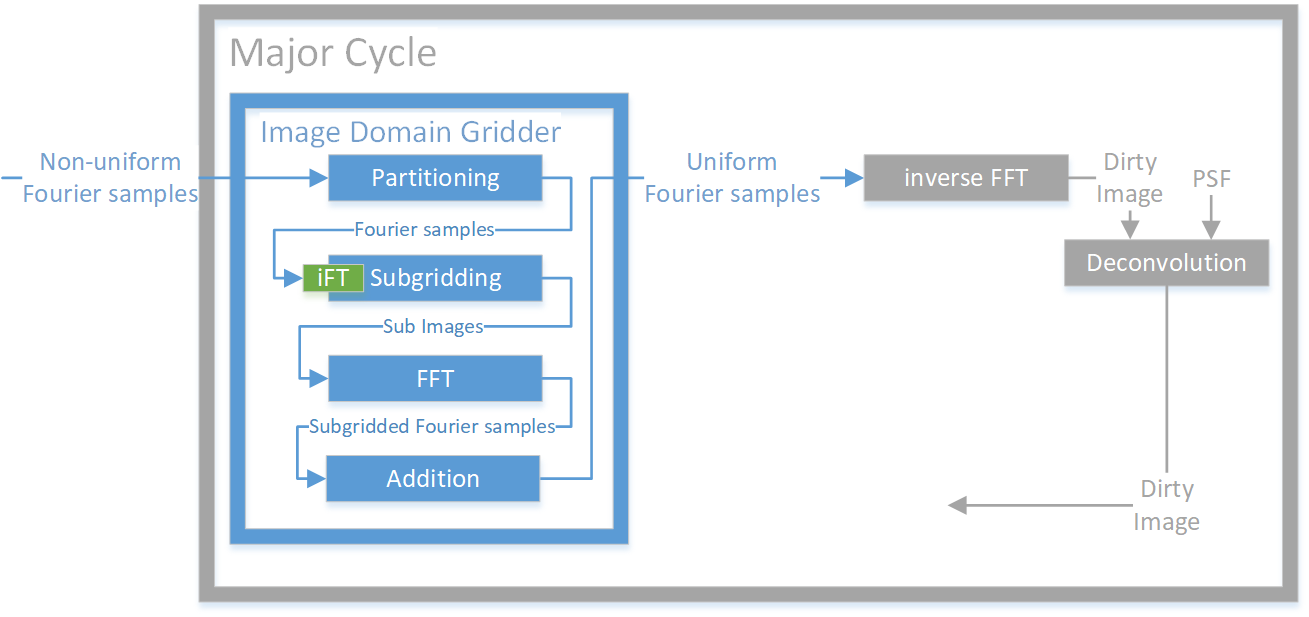
\includegraphics[width=0.80\linewidth]{./chapters/03.distribution/idg/major-minor-idg.png}
	\caption{Image Domain Gridder in the Major Cycle Architecture}
	\label{distribution:idg:system}
\end{figure}

Algorithm
\begin{figure}[h]
	\centering
	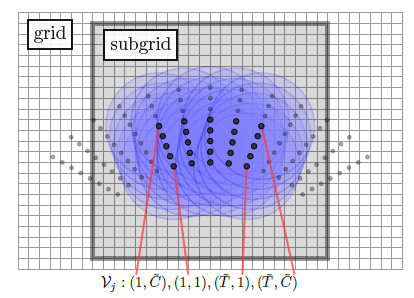
\includegraphics[width=0.40\linewidth]{./chapters/03.distribution/idg/subgrid.png}
	\caption{Subgrid}
	\label{distribution:idg:subgrid}
\end{figure}

\begin{figure}[h]
	\centering
	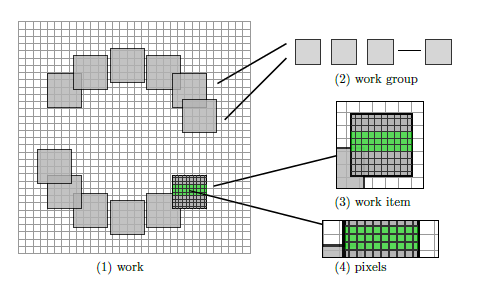
\includegraphics[width=0.40\linewidth]{./chapters/03.distribution/idg/paralellization.png}
	\caption{parallel}
	\label{distribution:idg:parallel}
\end{figure}

\begin{figure}[h]
	\centering
	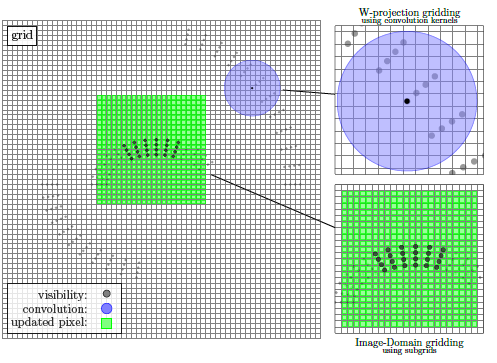
\includegraphics[width=0.40\linewidth]{./chapters/03.distribution/idg/idg0.png}
	\caption{Image Domain Gridder in the Major Cycle Architecture}
	\label{distribution:idg:idg0}
\end{figure}


\subsection{Deconvolution algorithms}
\subsubsection{MS-MFS-CLEAN}
CLEAN basic \cite{hogbom1974aperture}.

Latest variants for multiscale and multi frequency CLEAN (MS-MFS-CLEAN)\cite{rau2011multi}.

Current state-of-the-art

\subsubsection{MORESANE}
MORESANE \cite{dabbech2015moresane}


\subsection{Reconstruction algorithms which are not based on the deconvolution}
SARA\cite{dabbech2018cygnus}.











%\newpage
%\section{Coordinate descent deconvolution}\label{cd}
Coordinate descent methods are a family of algorithms. Various variants exist\cite{richtarik2016distributed, richtarik2016parallel}, but they share one common idea: Most of our problems become simple when we reduce the number of dimensions. Deconvolving a whole image is difficult. But deconvolving a single pixel is easy. As we will show in section \ref{cd:deriving}, we can derive a closed form solution\footnote{Deriving a formula which we can implement in a few lines of code.} for deconvolving a single pixel. We then iterate over all pixels, possibly several times, until we converge to a deconvolved image. 

This is the idea behind coordinate descent methods. By reducing the dimensions of the problem, we can often find an optimization algorithm where each iteration is "cheap" to compute. In these cases, coordinate descent methods produce competitive results\cite{nesterov2012efficiency, nesterov2013gradient}.

For a deconvolution algorithm in radio astronomy, we need three parts: An optimization algorithm, a regularization, and an optimization objective. We use coordinate Descent as the optimization algorithm, take Elastic Net as the regularization and use the following objective function:

\begin{equation}\label{cd:deconv}
\underset{x}{minimize} \: \frac{1}{2} \left \| I_{dirty} - x * PSF \right \|_2^2 + \lambda ElasticNet(x)
\end{equation}

As we have shown before, the objective function consists of two parts. The data term $\left \| I_{dirty} - x * PSF \right \|_2^2$ and the regularization term $ElasticNet(x)$. The data term forces the image to be as close to the measurements as possible which forces the image to be as close to the measurements as possible, the regularization term forces the image to be as consistent as possible with our prior knowledge. The parameter $\lambda$ is a weight that either forces more or less regularization. It is left to the user to define for each image. We will derive the coordinate descent algorithm that optimizes the objective \eqref{cd:deconv} in section \ref{cd:deriving}. First, let us explain what the elastic net regularization does.

\subsection{Elastic net regularization} \label{cd:reg}
\begin{figure}[h]
	\centering
	\begin{subfigure}[b]{0.3\linewidth}
		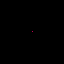
\includegraphics[width=\linewidth]{./chapters/03.distribution/L1.png}
		\caption{Effect of the pure L1 norm ($\lambda$ = 1.0) on a single point source.}
		\label{cd:elastic:L1}
	\end{subfigure}
	\begin{subfigure}[b]{0.3\linewidth}
		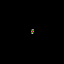
\includegraphics[width=\linewidth]{./chapters/03.distribution/L2.png}
		\caption{Effect of the pure L2 norm ($\lambda$ = 1.0) on a single point source.}
		\label{cd:elastic:L2}
	\end{subfigure}
	
	\caption{Effect of the L1 and L2 Norm separately.}
	\label{cd:elastic}
\end{figure}


This regularization is a mixture between the L1 and L2 regularization. The Figure \ref{cd:elastic} shows the effect of the L1 and L2 norm on a single star. The L1 regularization forces the image to contain few non-zero pixels as possible. It encodes our prior knowledge that the image will contain stars. The L2 regularization on the other hand "spreads" the single star across multiple pixels. This forces the image to represent extended emissions, like hydrogen cloud, with a large number of non-zero pixels (the L1 norm tends to break extended emissions apart, only using a handful of non-zero pixels). The L2 norm was already used in other image reconstruction algorithms in radio astronomy\cite{ferrari2014distributed}, with the downside that the resulting image will not be sparse.

Elastic net mixes these two norms together, becoming "sparsifying L2 norm". It retains the sparsifying property of the L1 norm, while also keeping extended emissions in the image. Formally, elastic net regularization is defined as the following:

\begin{equation}\label{cd:elastic:formula}
ElasticNet(x, \alpha) = \: \alpha \left \|x \right \|_1 + \frac{1-\alpha}{2}  \left \|x \right \|_2
\end{equation}

Elastic net has three properties which make it an interesting regularization for coordinate descent: It was shown to speed up convergence rates compared to the pure L1 or L2 norm\cite{friedman2010regularization}, is a separable function, and has a closed form solution. The first property was not further investigated in this work. The second property, separability, means that we can calculate the regularization for each pixel independently of each other, and we still arrive at the same result. Lastly, we can find a simple formula for each pixel that applies the elastic net regularization:

\begin{equation}\label{cd:elastic:closed}
ElasticNetClosedForm(x, \lambda ,\alpha) = \: \frac{max(x - \lambda * \alpha, 0)}{1+\lambda(1 - \alpha)}
\end{equation}

The closed form solution \eqref{cd:elastic:closed} of the elastic net regularization is also a mixture of the closed form solutions of the L1 and L2 norm. The closed form solution of the L1 norm is shrinkage: $max(x - \lambda, 0)$, we reduce the pixel value by $\lambda$ and clamp negative values. For the L2 norm, we divide the pixel value: $\frac{x}{1+\lambda}$.

%Proximal operator But the second property leads to an optimization algorithm 

Note that the shrink operation in this project always clamps negative pixels to zero. We constrain the image to only contain zero or positive pixel values. This has become a widely used constraint in radio interferometric image reconstruction and may lead to improved image quality\cite{mcewen2011compressed}.

Elastic net is the regularization we use throughout this work. It is separable (we can calculate it for each pixel independently) and has an easy to compute closed form solution.


\subsection{Deriving the basic coordinate descent deconvolution algorithm}\label{cd:deriving}
In this section we derive the basic coordinate descent deconvolution algorithm, which minimizes the objective \eqref{cd:deconv}. Coordinate descent methods have a tendency to need a more iterations to converge compared to other methods like gradient descent. However, when a single iteration is cheap to compute, they can be faster in practice\cite{shalev2011stochastic}. The elastic net regularization has an easy to compute closed form solution \eqref{cd:elastic:closed}, and a single iteration is cheap to compute.

We call the coordinate descent algorithm described here "basic". Other coordinate descent algorithms in the literature\cite{richtarik2016parallel,fercoq2015accelerated, richtarik2016distributed} can be seen as generalizations of the "basic" algorithm. The basic algorithm optimizes a single pixel at each iteration, while other algorithms can optimize one or several pixels. 
%We look at the basic coordinate descent algorithm first and use it as a baseline for comparing different coordinate descent algorithms.

In this section, we derive the basic coordinate descent algorithm that optimizes a single pixel in each iteration, and iterates over all pixels several times, with a specific strategy, until convergence. There are three types of iteration strategy we can choose:
\begin{enumerate}
	\item Random: where we choose a pixel to optimize uniformly at random.
	\item Greedy: where we first choose the pixel which minimizes our objective the most
	\item Cyclic: where we choose a subset of pixels and cycle through them until convergence. 
\end{enumerate}

The iteration strategy is not important for convergence. We can for example create a mixture of the different strategies and the algorithm would still converge to the optimum. However, the strategy we choose has an impact on how many iterations we need until convergence. For example: if the image consists of a single star in the center of the image, a greedy strategy would first optimize the pixel at the center, while a random strategy may waste the computing resources in checking every other pixel several times before finally landing on the center. In this implementation, we chose the greedy strategy. Each iteration takes the best possible step towards the optimum. We arrive at the following coordinate descent algorithm in pseudo code:


\begin{lstlisting}
dirty = IFFT(Gridding(visibilities))
residuals = dirty

x = new Array
objectiveValue = SUM(residuals * residuals) + P(x)
oldObjectiveValue = objectiveValue

do 
{
	oldObjectiveValue = objectiveValue

	//the core of the algorithm
	pixelLocation = GreedyStrategy(residuals)
	oldValue = x[pixelLocation]
	optimalValue = oldValue + Minimize(residuals, psf, pixelLocation)
	optimalValue = ApplyElasticNet(optimalValue, lambda, alpha)
	
	//housekeeping
	x[pixelLocation] = optimalValue
	residuals = residuals - PSF * (optimalValue - oldValue)
	objectiveValue = 0.5 * SUM(residuals * residuals) + lambda * ElasticNet(x, alpha)
} while (oldObjectiveValue - objectiveValue)  < epsilon
\end{lstlisting}

The core of the algorithm consists of the three functions: $GreedyStrategy()$, $Minimize()$ and $ApplyElasticNet()$. The function $GreedyStrategy()$ will be discussed in Section \ref{cd:efficient}. The function $ApplyElasticNet()$ was already described in equation \eqref{cd:elastic:closed}. The $Minimize()$ function is responsible for minimizing the data term of our objective \eqref{cd:deconv}. Because we only minimize a single pixel, we are dealing with a one dimensional minimization problem and can derive a closed form solution for it.

When we only have one pixel to minimize, the data term of our objective \eqref{cd:deconv} reduces itself to a parabola. We derive the standard parabola form in \eqref{cd:deriving:derivation}, where $\langle x, y\rangle$ is the inner product(element-wise multiplication followed by a sum over all elements):

\begin{equation} \label{cd:deriving:derivation}
\begin{split}
Minimize(pixel) & = \left \| I_{res} - PSF * pixel \right \|_2^2\\
Minimize(pixel) & = (I_{res} - PSF * pixel)^2\\
Minimize(pixel) & = \langle I_{res}, I_{res} \rangle - 2\langle I_{res},PSF\rangle * pixel + \langle PSF, PSF \rangle * pixel^2\\
Minimize(pixel) & = \langle PSF, PSF \rangle * pixel^2 - 2\langle I_{res},PSF\rangle * pixel + \langle I_{res}, I_{res} \rangle
\end{split}
\end{equation}

Now finding the optimal value for the pixel is the same as finding the optimal value of the parabola:

\begin{equation} \label{cd:deriving:minimizer}
\begin{split}
f(x) & = a*x^2 \\
 & + b*x \\
 & + c\\
 \\
x_{min} & = \frac{-b}{2a}
\end{split}
\quad \quad
\begin{split}
Minimize(pixel) & = \langle PSF, PSF \rangle * pixel^2 \\
 & - 2\langle I_{res},PSF\rangle * pixel \\
 &+ \langle I_{res}, I_{res} \rangle\\
 \\
pixel_{min} & = \frac{-(-2\langle I_{res},PSF\rangle)}{2\langle PSF, PSF \rangle}
\end{split}
\end{equation}

This means we can find the optimum value of a single pixel by following the formula in \eqref{cd:deriving:minimizer}. Note that the $PSF$ in formula \eqref{cd:deriving:derivation} and \eqref{cd:deriving:minimizer} is shifted to the pixel position we wish to optimize.

We derived the closed form solution \eqref{cd:deriving:minimizer} by looking at the data objective as a parabola. When we take another look at the closed form solution with Calculus in mind, we can see that the numerator $-2\langle I_{res},PSF\rangle)$ is actually the same as calculating the gradient for this pixel, and the denominator $\langle PSF, PSF \rangle$ is the Lipschitz constant. 

Intuitively, the Lipschitz constant describes how fast a function $f(x)$ changes with $x$. If $f(x)$ changes slowly, we can descend larger distances along the gradient without the fear for de-convergence. In short, it is a data-defined step size. Because our function $Minimize()$ is simply a parabola, the gradient together with the Lipschitz constant point to the optimum of our function.

Because the minimizer \eqref{cd:deriving:minimizer} of our coordinate descent algorithm calculates the gradient, one might ask what the differentiates the coordinate descent method from gradient descent. The main difference is that coordinate descent uses the gradient of a single pixel (or subset of pixels in other versions), in each iteration, while gradient descent generally uses the gradients of all pixels in each iteration. Conceptually, coordinate descent does is not bound to use the gradient. We could also minimize the pixel with a line-search algorithm, trying different values for the pixel, and it is still a coordinate descent method.

This is how the basic coordinate descent deconvolution algorithm works. But as it is described here, one iteration is too expensive to be practical. The $Minimize()$ function calculates both the gradient and the Lipschitz constant in each iteration and the residual update in line 20 requires a convolution. We can drastically improve the runtime costs by caching intermediate results, and using approximations.

\subsection{Efficient implementation of basic coordinate descent deconvolution}\label{cd:efficient}
In Section \ref{cd:deriving}, we derived the basic coordinate descent deconvolution algorithm. There are several "tricks" to speed up each iteration. We can cache intermediate results, and exploit the convolution to efficiently calculate the inner products of the basic algorithm We discuss:

\begin{enumerate}
	\item Edge handling of the convolution
	\item Pre-calculation of the Lipschitz constants
	\item Efficient greedy strategy
 	\item Pre-calculation of gradients
	\item Efficient update of gradients
\end{enumerate}

Gradient calculation is the most time consuming step. We can exploit the convolution to efficiently pre-calculate, update and approximate the gradients for each pixel. This will be discussed in detail in this Section. To our knowledge, we are the first to explore ways to approximate the gradient in radio interferometric image reconstruction, and their effect on parallel and distributed deconvolution. As we will se in the later sections, approximating the gradients can help us to distribute the deconvolution. 

Visual aid:
\begin{figure}[h]
	\centering
	\begin{subfigure}[b]{0.3\linewidth}
		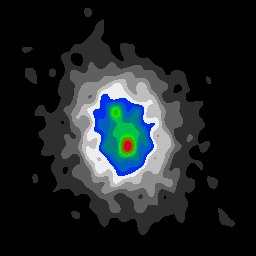
\includegraphics[width=\linewidth]{./chapters/03.distribution/simulated/dirty.png}
		\caption{Dirty Image.}
		\label{cd:efficient:aid:dirty}
	\end{subfigure}
	\begin{subfigure}[b]{0.3\linewidth}
		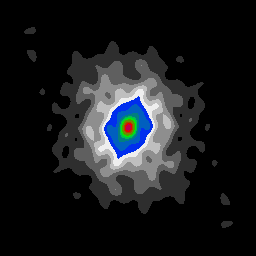
\includegraphics[width=\linewidth]{./chapters/03.distribution/simulated/psf.png}
		\caption{Point Spread Function.}
		\label{cd:efficient:aid:psf}
	\end{subfigure}
	\begin{subfigure}[b]{0.3\linewidth}
		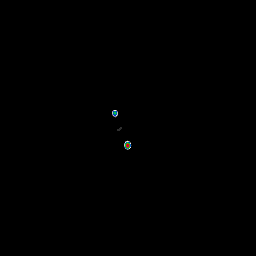
\includegraphics[width=\linewidth]{./chapters/03.distribution/simulated/elastic.png}
		\caption{ElasticNet deconvolution}
		\label{cd:efficient:aid:elastic}
	\end{subfigure}
	
	\caption{Example problem with two point sources.}
	\label{cd:efficient:aid:figure}
\end{figure}

First, we dive into the implementation of the convolution operator and the pre-calculation of the Lipschitz constants, and then we discuss the gradient calculation in detail.

\subsubsection{Edge handling of the convolution}
As the reader is probably aware, there are several ways to define the convolution in image processing, depending on how we handle the edges on the image. Two possibilities are relevant for radio interferometric image reconstruction: Circular and zero padded.

\begin{figure}[h]
	\centering
	\begin{subfigure}[b]{0.3\linewidth}
		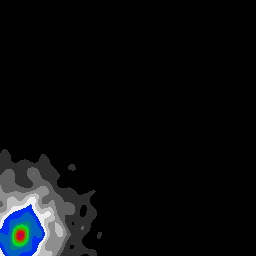
\includegraphics[width=\linewidth]{./chapters/03.distribution/simulated/padded.png}
		\caption{Zero padded convolution.}
		\label{cd:efficient:convolution:padded}
	\end{subfigure}
	\begin{subfigure}[b]{0.3\linewidth}
		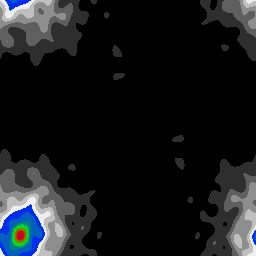
\includegraphics[width=\linewidth]{./chapters/03.distribution/simulated/circular.png}
		\caption{Circular convolution.}
		\label{cd:efficient:convolution:circular}
	\end{subfigure}
	\caption{Comparison of the two convolution schemes.}
	\label{cd:efficient:convolution:figure}
\end{figure}

Circular convolution assumes the image "wraps" around itself. If we travel over the right edge of the image, we arrive at the left edge. The convolution in Fourier space is circular. Remember: A convonlution in image space is a multiplication in Fourier space, and vice versa. When we convolve the reconstructed image $x$ with the $PSF$ using circular convolution, then non-zero pixels at the right edge of the image "shine" over to the left edge. This is physically impossible.

Zero padding assumes that after the edge, the image is zero. Non-zero pixels at the right edges of the image do not influence the left edge after convolution. This is the physically plausible solution. However, the zero padded convolution is more expensive to calculate. We either have to calculate the convolution in image space, which is too expensive for large kernels, or apply the FFT on a zero-padded image. Either way, it is more expensive than the circular convolution.

In designing a deconvolution algorithm, we have the choice between the circular and the zero-padded convolution scheme. Circular convolution is more efficient to calculate, while zero-padded convolution is closer to the reality. Both choices are possible. The PyMORESANE reconstruction algorithm \cite{kenyon2019pymoresane} leaves this choice to the user. We decided on using the zero-padded convolution. This choice influences other parts of the coordinate descent deconvolution algorithm, like how we can efficiently calculate the Lipschitz constants.

\subsubsection{Pre-calculation of the Lipschitz constants}
Lipschitz constants are $\langle PSF, PSF \rangle$. We simply multiply the $PSF$ with itself and sum up the values. However, we are using the zero-padded convolution. This means the $PSF$ for pixels at the edges is not only shifted, but also cropped. In other words, every pixel has a different Lipschitz constant depending on how much the $PSF$ gets cropped by the image edges.

Note that it is not an issue for convergence: The Lipschitz constant describes the largest step we can take without overshooting the target. We can always make smaller steps, but may pay it with more iterations. The Lipschitz constant of the edge pixels is always lower than the center. The coordinate descent algorithm does converge, but needs more iterations for pixels at the edges of the image. Luckily, there is a way to re-use intermediate results, and efficiently calculate the Lipschitz constant for each pixel in the image.

The first observation is that the image edges always create a rectangular crop of the $PSF$. To calculate the Lipschitz constant, we square and sum up all the values that lie inside the rectangle. This can be exploited with a scan algorithm: We store the $PSF$ as a running sum of squares. 

\begin{lstlisting}
var scan = new double[,];
for (i in (0, PSF.Length(0))
{
	for (j in (0, PSF.Length(1))
	{
		var iBefore = scan[i - 1, j];
		var jBefore = scan[i, j - 1];
		var ijBefore = scan[i - 1, j - 1];
		var current = PSF[i, j] * PSF[i, j];
		scan[i, j] = current + iBefore + jBefore - ijBefore;
	}
}
\end{lstlisting}

$scan[0, 13]$ contains the sum of the squared $PSF$ values from index $(0,0)$ up to and including index $(0, 13)$. The last element, $scan[PSF.Length(0) - 1, PSF.Length(1) -1]$ contains the sum of squares over the whole $PSF$. In short, we have stored the sum of all possible rectangles starting from index $(0,0)$. If a part of the $PSF$ is cropped, we can look up $scan$ and find out by how much it affects the total sum.

Up to 4 

%Numerical issues with float precision.

\subsubsection{Efficient Greedy strategy}

Calculate what each update would lead to what objective.
Expensive to calculate.

However, we can use another strategy, we use the biggest change in pixel value.
A lot cheaper to compute
Biggest change in pixel value is in toy examples the same as the best pixel. 

Not sure if this is always true.


\subsubsection{Pre-calculation of gradients}
In each iteration, we need to know the gradient for all pixels. We need to calculate the inner product $\langle I_{res},PSF\rangle$ for each pixel. Typically, the $PSF$ and the image have the same number of pixels, which leads to a quadratic number of operations to calculate all gradients.

Luckily, we can use the Fourier transform to speed up the calculation. Notice that the inner product $\langle I_{res},PSF\rangle$ is equivalent to calculating the correlation of the residuals with the $PSF$ ($)I_{res} \star PSF$). The convolution and correlation operators are related: The convolution is equal to a correlation with a flipped kernel. Since a convolution in image space is a multiplication in Fourier space, we can calculate the $PSF$ correlation efficiently in Fourier space.

\begin{figure}[h]
	\centering
	\begin{subfigure}[b]{0.3\linewidth}
		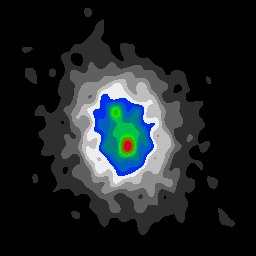
\includegraphics[width=\linewidth]{./chapters/03.distribution/simulated/dirty.png}
		\caption{Dirty Image.}
		\label{cd:efficient:gradients:dirty}
	\end{subfigure}
	\begin{subfigure}[b]{0.3\linewidth}
		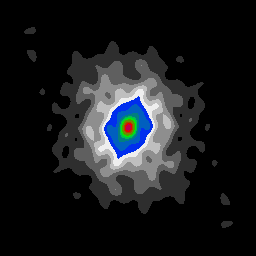
\includegraphics[width=\linewidth]{./chapters/03.distribution/simulated/psf.png}
		\caption{Point Spread Function.}
		\label{cd:efficient:gradients:psf}
	\end{subfigure}
	\begin{subfigure}[b]{0.3\linewidth}
		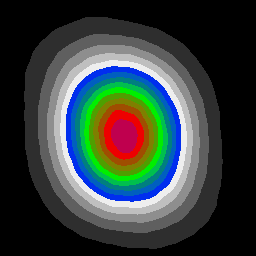
\includegraphics[width=\linewidth]{./chapters/03.distribution/simulated/gradients.png}
		\caption{Gradient for each pixel.}
		\label{cd:efficient:gradients:gradients}
	\end{subfigure}
	
	\caption{Example of the gradient calculation.}
	\label{cd:efficient:gradients:figure}
\end{figure}

The Figure \ref{cd:efficient:gradients:figure} shows the process for the first step of the coordinate descent deconvolution. We start with the dirty image. We calculate the correlation of the $PSF$ with the dirty image and arrive at the map of gradients. Figure \ref{cd:efficient:gradients:gradients} shows the gradient for each pixel.

\subsubsection{Efficient update of gradients}
The naive coordinate descent implementation minimizes a single pixel, and updates the residuals by subtracting the $PSF$ at the correct location (The first line of \eqref{cd:efficient:update:naive}). It then calculates the new gradient for each pixel(Second line of \eqref{cd:efficient:update:naive}) in each iteration. This is not necessary. We only need to calculate the correlation in the first iteration. All later iterations update the map gradients directly without the Fourier transform.

\begin{equation}\label{cd:efficient:update:naive}
\begin{split}
residuals &= residuals - PSF * (optimalValue - oldValue) \\
gradients &= residuals \star PSF
\end{split}
\end{equation}

The trick is to combine both lines of the naive update \eqref{cd:efficient:update:naive}. We correlate each term of the first line with the $PSF$, and we arrive at the update rule \eqref{cd:efficient:update:new}.

\begin{equation}\label{cd:efficient:update:new}
gradients = gradients - (PSF \star PSF) * (optimalValue - oldValue)
\end{equation}

The noteworthy part of \eqref{cd:efficient:update:new} is that we update the gradients directly, but instead of using the $PSF$, we take the product of $(PSF \star PSF)$, of the $PSF$ correlated with itself. Also note that we do not need to keep the residuals in memory. All we need is the map of gradients. 

\begin{figure}[!h]
	\centering
	\begin{subfigure}[b]{0.3\linewidth}
		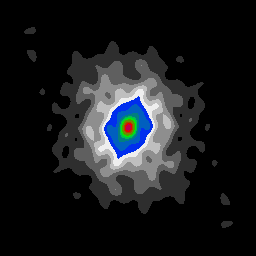
\includegraphics[width=\linewidth]{./chapters/03.distribution/simulated/psf.png}
		\caption{Point Spread Function.}
		\label{cd:efficient:update:dirty}
	\end{subfigure}
	\begin{subfigure}[b]{0.3\linewidth}
		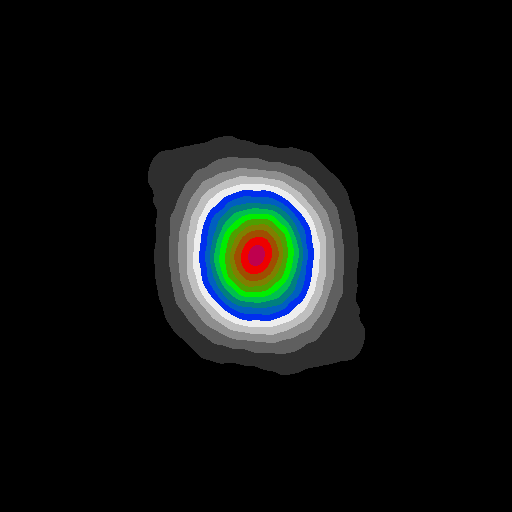
\includegraphics[width=\linewidth]{./chapters/03.distribution/simulated/psf2.png}
		\caption{Gradient update: $(PSF \star PSF)$.}
		\label{cd:efficient:update:psf}
	\end{subfigure}
	\caption{Example problem with two point sources.}
	\label{cd:efficient:update:figure}
\end{figure}

Calculate the PSF correlation with itself. Calculate the PSF correlation once, and use it to update the gradient map directly.

Edges again. We have the problem that, when the PSF is cutoff by the edges of the image, we would need to calculate $(PSF \star PSF)$ again. This is too expensive. Does not change dramatically, unless the pixel we optimize is at the full edge.


\subsection{Similarities to the CLEAN algorithm}

Comparison to CLEAN. Similar algorithm, but we descend in the actual gradient direction.

\subsection{Pseudo-code of the basic, optimized algorithm}

putting it all together




GPU implementation




\subsection{Distributed Deconvolution}
How do we distribute the major cycle. We need to distribute every step, Gridding, FFT and Deconvolution.

Gridding, Large number of input data. This needs to be distributed
We use the Image domain gridding introduces in sectionand use it as the basis for the distributed gridding.

The FFT is generally not worth distributing, if we can keep all the data in memory. When the gridding is done, in our setup, the grid is small enough to keep in memory. (cite distributed fftw)

Deconvolution is also worth distributing. CLEAN depending on the observation is the second most time consuming step. But gridding tends to be easier to distribute, so in some observations it is the most time consuming step.
Split the image into patches and deconvolve each patch.
Sadly not possible, we need communication. how we communicate is important.

We use a distributed Gridding and a distributed deconvolution. Which leads us to the following architecture.

\begin{figure}[h]
	\centering
	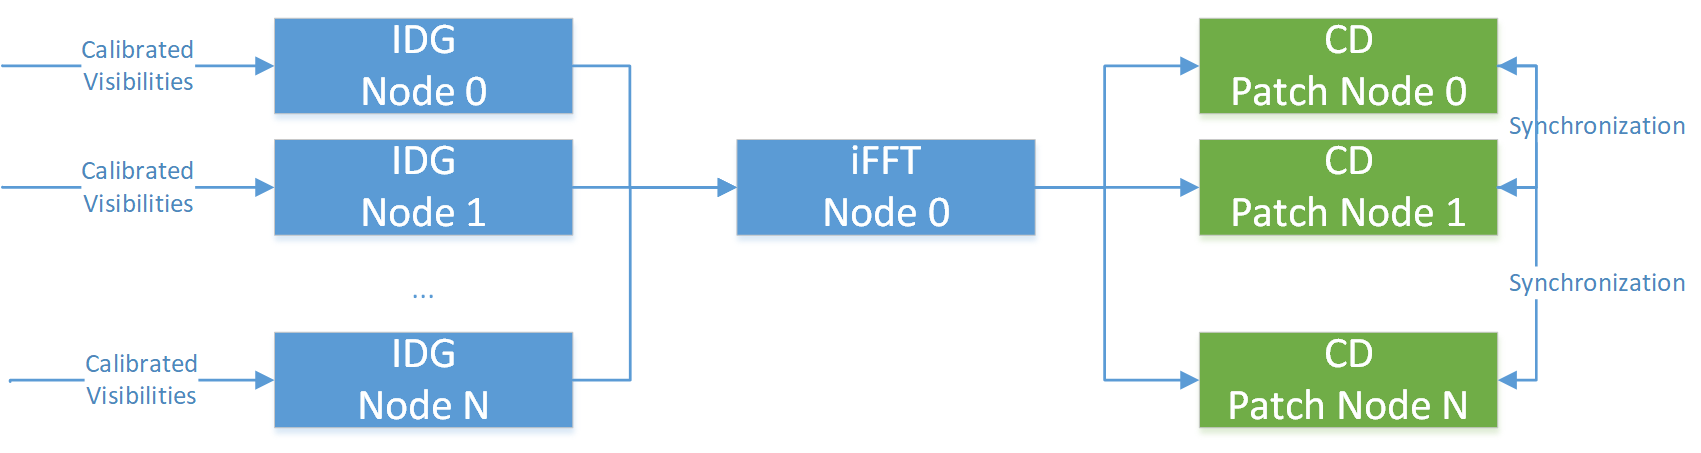
\includegraphics[width=0.80\linewidth]{./chapters/03.distribution/distributed_architecture.png}
	\caption{Distributed architecture for half a major cycle}
	\label{dist:architecture:fig}
\end{figure}

Where each node is one computer, i.e. has its own, possibly multiple cpus and its shared memory.
Split the input visibilities onto nodes. 
Do the gridding locally on each node
Communicate the grid
inverse FFT on one node.
Communicate the patches of the image.
Deconvolve each patch and communicate


\newpage
\bibliography{mybib}{}
%\bibliographystyle{plain}
\bibliographystyle{unsrt}
\newpage
%\listoffigures
%\listoftables

%\end{multicols}

\newpage
%\pagebreak
\section{Attachment}

\subsection*{Parameters of the WSCLEAN}
Parameters of multi-scale CLEAN
\begin{lstlisting}
wsclean -multiscale -data-colun DATA --niter 34000 -padding 1.5 -size 3072 3072 -scale 1.5asec -mgain 0.8 -gain 0.1 -auto-threshold 3 -auto-mask 5
\end{lstlisting}

Parameters of MORESANE (IUWT)
\begin{lstlisting}
wsclean -iuwt -data-colun DATA --niter 200 -padding 1.5 -size 3072 3072 -scale 1.5asec -mgain 0.4 -gain 0.2 -auto-threshold 1.5 -auto-mask 2
\end{lstlisting}


\subsection*{Serial coordinate descent algorithm}

\subsubsection*{Efficient calculation of the Lipschitz constants}
In each iteration, we need the Lipschitz constant of the current pixel. I.e. we need the inner product $\langle PSF_{location}, PSF_{location} \rangle$ for every pixel. We can pre-calculate the Lipschitz constant before we run the serial coordinate descent algorithm. The naive way to calculate the Lipschitz constant for every pixel results in quadratic runtime(each inner product costs us $O(n)$ operations, and we do it for all $n$ pixels). But this is not necessary. We can pre-calculate the Lipschitz constant for every pixel in linear time.

Figure \ref{cd:efficient:lipschitz:padded} shows the $PSF$ shifted to a pixel location. The Lipschitz constant is by squaring all values of Figure \ref{cd:efficient:lipschitz:padded} and summing up the values. Or in another way: We sum up all the squared values of the $PSF$ inside a specific rectangle. All that changes for a Lipschitz calculation between different pixels is the specific rectangle.

\begin{figure}[h]
	\centering
	\begin{subfigure}[b]{0.3\linewidth}
		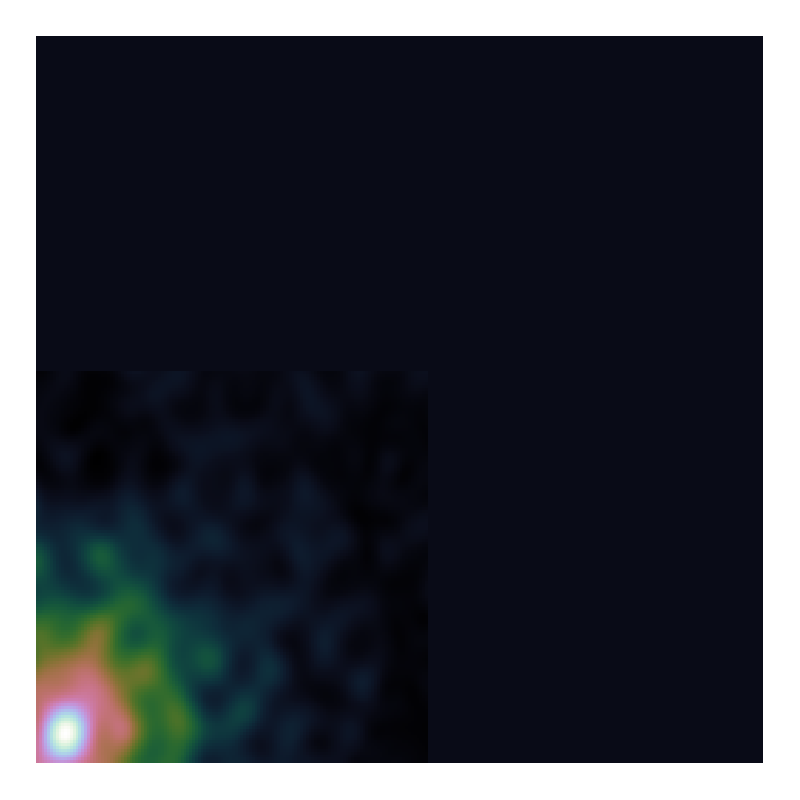
\includegraphics[width=\linewidth, clip, trim= 0.25in 0.25in 0.25in 0.25in]{./chapters/03.cd/simulated/psfZeroPadding.png}
		\caption{Shifted $PSF$.}
		\label{cd:efficient:lipschitz:padded}
	\end{subfigure}
	\begin{subfigure}[b]{0.3\linewidth}
		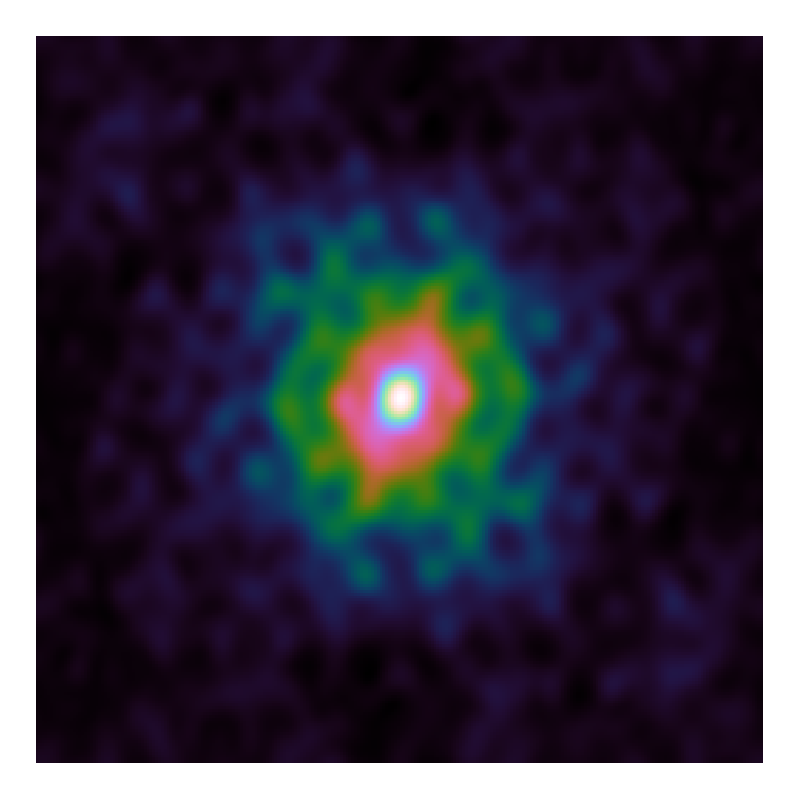
\includegraphics[width=\linewidth, clip, trim= 0.25in 0.25in 0.25in 0.25in]{./chapters/03.cd/simulated/psf.png}
		\caption{Sum of squared values.}
		\label{cd:efficient:lipschitz:rectangle}
	\end{subfigure}
	\caption{Sum of squared values for the Lipschitz constant.}
	\label{cd:efficient:lipschitz:figure}
\end{figure}

This can be exploited with a scan algorithm: We first calculate the result of every rectangle we can draw from the origin, up to some pixel value. We end up with an array we call $scan[,]$. It is the same size as the $PSF$, but contains the sum of squares inside a specific rectangle.

\begin{lstlisting}
var scan = new double[,];
for (i in (0, PSF.Length(0))
for (j in (0, PSF.Length(1))
var iBefore = scan[i - 1, j];
var jBefore = scan[i, j - 1];
var ijBefore = scan[i - 1, j - 1];
var current = PSF[i, j] * PSF[i, j];
scan[i, j] = current + iBefore + jBefore - ijBefore;
\end{lstlisting}

Every Lipschitz constant can be now calculated by combining the sums of different rectangles. Our example is shown in Figure \ref{cd:efficient:lipschitz:rectangle}. We start with the total sum of all values, and subtract two rectangles. Because the subtractions overlap, we need to add the third rectangle again. we take the total value. In short, we can calculate each Lipschitz constant by at most 4 lookups in the $scan[,]$ array.


\subsubsection*{GPU implementation}
We implemented the serial coordinate descent algorithm on the GPU. It is implemented in .Net Core with ILGPU\cite{ilgpu}. ILGPU is a Just-In-Time compiler for high performance GPU programs written in .Net Core.

GPU programs are split into kernels. Each kernel consists of a single routine optimized for executing on the GPU. Our serial coordinate descent algorithm consists of Step 1, find the best pixel to optimize, step 2, optimize pixel and then updating the gradient map. The GPU implementation of the Serial coordinate descent algorithm uses three kernels: Kernel 1 is equivalent to step 1. Kernel 2 updates the reconstruction $x$ and kernel 3 updates the gradient map.

Kernel 2 and 3 are straight forward to implement. The implementation of kernel 1, searching for the best pixel, is more interesting. Essentially, this step is a max reduce operation: We want to find the pixel with the maximum absolute step. We implemented the step 1 kernel with an atomic-max instruction:
\begin{lstlisting}
MaxPixelKernel(x, gradienstMap, lipschitz, location, maxPixel)
oldValue = x[location]
tmp = gradientsMap[location] + oldValue * lipschitzMap[location]
optimalValue = Max(tmp - lambda*alpha) / (lipschitz[location] + (1 - alpha)*lambda)
diff = optimalValue - oldValue
currentPixel = (absDiff = Abs(diff), diff = diff, location = location)
AtomicMax(maxPixel, currentPixel)
\end{lstlisting}

The kernel is executed on multiple processors in parallel on the GPU. Each processor is checking a single pixel. Communication is done with the atomic-max instruction. The atomic-max writes on a global variable, which keeps track of the current maximum pixel. This implementation turned out to be the fastest for the MaxPixelKernel. Warp shuffle\cite{keplerShuffle} was also tested, but resulted in a slower kernel.

Now to put the serial coordinate descent implementation on the GPU together, all we need to do is call the kernels, which perform the minimization on the GPU:


\begin{lstlisting}
do 
//Step 1: Search pixel
maxPixel = (absDiff = 0, diff = 0, location = (-1, -1))
ExecuteMaxPixelKernel(x, gradienstMap, lipschitz, maxPixel)
SynchronizeKernels()

//Step 2: Optimize
ExecuteUpdateXKernel(x, maxPixel.diff, maxPixel.location)
ExecuteUpdateGradientsKernel(gradientsMap, gradientUpdate, maxPixel.diff, maxPixel.location)
SynchronizeKernels()

while maxPixel.absDiff  < epsilon
\end{lstlisting}

Note that after each kernel call, we synchronize the program. We wait for all kernels on the GPU to be finished, before we continue with the next step. As we mentioned before, this is the core behind the serial coordinate descent algorithm. We have to wait for each step to finish before we can continue with the next. 


\subsubsection*{Distributed implementation MPI}
We created a distributed implementation of our serial coordinate descent algorithm using the Message Passing Interface (MPI). In MPI, we use several nodes of computers to solve the problem. Each node has its own processors an main memory, and we use MPI to communicate betweeen the nodes. 

We split the reconstructed image, and the gradient map into facets of equal size, and use one node for each facet. For example, our image is $1024^2$ pixels in size and we use 4 nodes. This means each node reconstructs a $512^2$ facet of the image, and has the matching $512^2$ entries of the gradient map locally. 

The distributed serial coordinate descent algorithm now searches the maximum pixel locally in each node. Then, all node agree on the best global pixel to optimize, which is an MPI\_ALLREDUCE operation. After MPI\_ALLREDUCE, each node knows the global pixel which gets minimized in this iteration. Then, each node updates its part of the gradient map locally.

This leads to the following pseudo-code algorithm:
\begin{lstlisting}
...
do 
oldObjectiveValue = objectiveValue

//Step 1: Search pixel
maxAbsDiff = 0
maxDiff = 0
pixelLocation = (-1, -1)
for(i in Range(0, dirty.Length(0))
for(j in Range(0, dirty.Length(1))
oldValue = x[i, j]
tmp = gradientsMap[i, j] + oldValue * lipschitzMap[i, j]
optimalValue = Max(tmp - lambda*alpha) / (lipschitz[i, j] + (1 - alpha)*lambda)
diff = optimalValue - oldValue

if(maxAbsDiff < Abs(diff))
maxAbsDiff = Abs(diff)
maxDiff = diff
pixelLocation = (i, j)

//communicate location with nodes
globalMaxAbsDiff, globalMaxDiff, globalLocation = MPI_ALLREDUCE(maxAbsDiff, maxDiff, pixelLocation)

//Step 2: Optimize pixel.
if(globalLocation == pixelLocation)
x[globalLocation] += globalMaxDiff

//housekeeping
shiftedUpdate = Shift(gradientUpdate, globalLocation)
gradientMap = gradientMap - shiftedUpdate * globalMaxDiff
while epsilon < maxAbsDiff
\end{lstlisting}

Each node in the distributed serial coordinate descent algorithm communicates its local pixel in each iteration. Meaning the distributed algorithm has a communication step in each serial coordinate descent iteration. The distributed algorithm only has to communicate a single pixel, but has to communicate often. This is a potential down-side of the implementation. Usually, distributed systems can speed up algorithms which communicate a large chunk of data rarely.

\subsubsection*{Serial coordinate descent speedup with MPI or GPU}\label{results:speedup}
In this section we test how much we can speed-up our serial coordinate descent algorithm by using distributed computing with MPI, or GPU acceleration.

We test the distributed serial coordinate descent on a shared memory system(Meaning all CPUs have access to the same main memory) with 32 CPUs. This is a best-case scenario for our implementation, because each node runs on the same physical machine: Our implementation needs a communication step between the nodes for each serial coordinate descent iteration. It needs a low-latency connection between each node to run as efficient as possible. Since each node runs on the same physical machine, it has a low latency times and therefore a low communication time. In this implementation, each node uses a single processor. We compare the speedup the algorithm achieves by adding more nodes/processors.

For the GPU we used personal computer level hardware, and tested on a nVidia Quadro M1200. We compare the speedup we achieve to the on-board CPU, which is an Intel Xeon E3-1505M with 8 logical processors at different image sizes. The speedup is shown in Figure \ref{results:speedup:figure}.

\begin{figure}[h]
	\centering
	\begin{subfigure}[b]{0.45\linewidth}
		\includegraphics[width=1.00\linewidth]{./chapters/10.results/speedup/dist-speedup.png}
	\end{subfigure}
	\begin{subfigure}[b]{0.45\linewidth}
		\includegraphics[width=1.00\linewidth]{./chapters/10.results/speedup/gpu.png}
	\end{subfigure}
	\caption{Speedup by using MPI or GPU acceleration}
	\label{results:speedup:figure}
\end{figure}

As we mentioned before, the speedup we achieve by using nodes/processors in MPI is the best-case scenario. As the best case scenario, we achieve a significant performance increase by using more nodes/processors. Up to 16 processors, the speedup we achieve is at least linear. Afterwards however the speedup diminishes. With 32 processors, we are only marginally faster than with 16. If the nodes would run two different physical machines, the speedup we achieve would depend mainly on the latency of the connection. 

The speedup we achieve by using GPU acceleration is fairly constant over the image size. The speedup factor varies around 2.5. Ideally, we would like to combine the distributed and the GPU implementation. However, this is not useful with the current implementation: The main bottleneck in the MPI implementation is the communication step in each iteration. 

We do not have a CLEAN implementation in our .Net Core pipeline. However, we mentioned the similarities between the serial coordinate descent and CLEAN in Section \ref{cd:similarities}. A single serial coordinate descent iteration is roughly equivalent to a standard CLEAN iteration. If we assume we need 14'000 CLEAN iterations to reconstruct an image, we can get a rough estimate by comparing the wall-clock time of 14'000 serial coordinate descent iterations. In this case, CLEAN is roughly 7 times faster than the current serial coordinate descent iteration.

Overall the serial coordinate descent algorithm with GPU acceleration is still several factors slower than CLEAN. The speedup we achieve with MPI is significant. But because serial coordinate descent and CLEAN have such a similar structure, we can expect a similar speedup with a CLEAN-MPI implementation. We need another method to speed up our deconvolution algorithm.


\subsection*{Parallel coordinate descent algorithm}

\subsubsection*{Block coordinate descent}
Instead of optimizing a single pixel in each iteration, the serial block coordinate descent algorithm can update a block of pixels. We start with the update rule of the serial coordinate descent algorithm, and show how it can be adapted to update a block of pixels in each iteration. Remember the single pixel update from the serial coordinate descent algorithm: 
\begin{equation} \label{pcdm:pcdm:block:single:update}
pixel_{opt} = \frac{max(gradient_{location} - \lambda\alpha, 0)}{Lipschitz_{location} + (1 - \alpha)\lambda}
\end{equation}

We optimize the pixel at the current location by taking the gradient and dividing it by the Lipschitz constant. For the block coordinate descent algorithm we vectorize the update rule: This means $gradient_{location}$ and $Lipschitz_{location}$ and the output $pixel_{opt}$ become vectors:

\begin{equation} \label{pcdm:pcdm:block:block:update}
pixels_{opt} = \frac{max(gradients_{locations} - \lambda\alpha, 0)}{Sum(Lipschitz_{locations}) + (1 - \alpha)\lambda}
\end{equation}

This is the serial block coordinate descent update rule. Note that we divide the gradient for each pixel by the the block Lipschitz constant (which is the sum of every pixel Lipschitz constant in the block). Note that the larger block we chose, the smaller the update becomes for each individual pixel inside the block. We have a central trade-off: We can take a large step for a single pixel, or take several smaller steps for a block of pixels. 

Remember: The Lipschitz constants for neighboring pixels have a similar value. Meaning for a block of $2^2 = 4$ pixels: $Sum(Lipschitz_{locations} \approx 4 Lipschitz$. Or less formally, we can either take a full step towards the minimum for a single pixel. Or if we update a block of $2^2$ pixels, we take $4$ $\frac{1}{4}$ steps towards the minimum.

The reader might be familiar with the (F)ISTA method\cite{beck2009fista}. The block update shown in equation \eqref{pcdm:pcdm:block:block:update} is related to the (F)ISTA update rule. When the block size equal to the image size (we update all pixels in the image in each iteration), then the serial block coordinate descent is equivalent to (F)ISTA.

The block update rule \eqref{pcdm:pcdm:block:block:update} allows us to minimize a single block of pixels in each iteration. But it comes with a trade-off: The bigger blocks we choose, the smaller steps we take for each individual pixel in the block. The reason why the serial block coordinate descent may be faster than the single pixel algorithm is when most pixels are correlated with their neighbors: Extended emissions have a large areas where the pixel values are correlated. Meaning if a pixel in the area is non-zero, then the neighboring pixels are also likely to be non-zero. A serial block coordinate descent algorithm can take more useful minimization steps in each iteration. We test different block sizes with our parallel algorithm in Section \ref{pcdm:results}. In our tests, different block sizes did not lead to a significant speedup.

\subsubsection*{Accelerated parallel block coordinate descent} \label{pcdm:pcdm:approx}
So far, we introduced the serial block coordinate descent and the ESO. The serial block coordinate descent can update a block of pixels in a single iteration, and the ESO estimates how much $PSF$s overlap when we perform parallel update steps. In this section, we put this together in an accelerated, parallel block coordinate descent algorithm based on APPROX\cite{fercoq2015accelerated}. But first, we introduce gradient acceleration.

In gradient acceleration, we use the gradient from previous iterations to speed up convergence of the current iteration. We can accelerate our serial coordinate descent algorithm by extending it with an acceleration parameter $\theta$, a copy of the gradient map and a copy of the reconstructed image $x$.  We term one couple of gradient map plus reconstructed image as 'explore', while the other couple is called 'correction'. The 'correction' gradient map and reconstructed image contain gradient information of the previous iterations. They are used to speed up the convergence of the 'explore'. In each iteration, the acceleration parameter $\theta$ decreases, and we use more information from the 'correction' gradient map and reconstruction.

This leads to the following accelerated, parallel and block coordinate descent deconvolution algorithm:
\begin{lstlisting}
dirty = IFFT(GridVisibilities(visibilities))
residualsPadded = ZeroPadding(dirty)

psfPadded = ZeroPadding(PSF)
psfPadded = FlipUD(FlipLR(psfPadded))
gradientUpdate = iFFT(FFT(ZeroPadding(PSF)) * FFT(psfPadded))

xExplore = new Array[,]
xCorrection = new Array[,]
gradientsMapExplore = iFFT(FFT(residualsPadded) * FFT(psfPadded))
gradientMapCorrection = new Array[,]
lipschitzMap = CalcLipschitz(PSF)

eso = ESO(CountNonZero(PSF), t, x.Length / blockSize)
theta0 = t / (x.Length / blockSize)
theta = theta0

do 
oldObjectiveValue = objectiveValue

//Step 1: select t blocks uniformly at random
blocks = sample(t)

//Step 2: update reconstruction in parallel
diffBlocks = new Array
parallel for each block in blocks
//increase blockLipschitz according to the ESO
blockLipschitz = Sum(GetBlock(LipschitzMap, block))
blockLipschitz = blockLipschitz * eso

oldBlock = GetBlock(xExplore, block)
tmp = theta^2 * GetBlock(gradientsMapCorrection, block) 
+ GetBlock(gradientsMapExplore, block) 
+ GetBLock(xExplore, block) * blockLipschitz
optimalBlock = Max(tmp - lambda*alpha) / (blockLipschitz + (1 - alpha)*lambda)
diffBlock = optimalBlock - oldBlock

xExplore[block] += diffBlock
xCorrection[block] += diffBlock * (-(1.0f - theta / theta0) / theta^2)
diffBlocks[block] = diffBlock

//Step 3: Update gradients
for each block in blocks
diffBlock = diffBlocks[block]
for each pixel in block
diff = diffBlock[pixel]
shiftedUpdate = Shift(gradientUpdate, pixelLocation)

gradientsMapExplore = gradientsMapExplore - shiftedUpdate * diff
gradientsMapCorrection = gradientsMapCorrection - shiftedUpdate * diff * (-(1.0f - theta / theta0) / theta^2)

theta = (Sqrt((theta^2 * theta^2) + 4 * (theta^2)) - theta^2) / 2.0f
while maxAbsDiff  < epsilon

output = new float[,]
for(i in in Range(0, dirty.Length(0))
for(j in in Range(0, dirty.Length(0))
output[i, j] = theta * xCorrection[i, j] + xExplore[i, j];
\end{lstlisting}

In each iteration, the parallel algorithm first samples $\tau$ unique blocks uniformly at random (we cannot select the same block more than in a single iteration). In the second step, we then update each block in parallel. Note that we multiply the block Lipschitz constant with the ESO, which ensures convergence for parallel updates. In the third step, we update the two gradient maps. The final image is a combination of the two reconstructed images $x$ from the 'explore' and 'correction' couple.

This algorithm is parallel, but it is still synchronized: It updates each block in parallel, but waits for all updates to finish before continuing with the next iteration. In the next Section \ref{pcdm:async}, we introduce an asynchronous implementation, where the individual processors do not wait for each other.

The accelerated, parallel coordinate descent algorithm reduces itself to a non-accelerated variant, if we do not modify $\theta$ in each iteration. In that case, the 'correction' gradient map and reconstruction $x$ stay zero over the course of the algorithm. Note that due to gradient acceleration, we need twice the memory (for the 'correction' maps), and twice the number of operations to update a single block. Gradient acceleration allows us to take larger steps towards the optimum in each iteration. As such, it should need fewer iterations to converge than the non-accelerated variant. But a single iteration of the accelerated variant is more expensive.

\subsubsection*{Active set heuristic}
The active set heuristic is typically used in cyclic coordinate descent: It chooses a subset of blocks, and optimizes the set until it converges. Then it chooses a  new set. We use the active set heuristic together with our pseudo-random selection strategy. A large portion of the blocks in the image will be zero. If we select blocks at pseudo-random, we are likely to select a block that will never contain non-zero values and we wasted computing resources by trying to update this block. The active set heuristic increases the likelihood that the pseudo-random strategy selects a relevant block. 

At the start of the parallel deconvolution algorithm, we initialize the active set by iterating over all blocks. We add all blocks which contain non-zero pixels, or pixels which may become non-zero by a serial coordinate descent iteration. Now during asynchronous parallel coordinate descent iterations, each processors only selects blocks from the active set. This increases the chance that each processor selects a block where pixel values can actually be modified.

Note that the algorithm only adds blocks to the active set, which can be changed to a non-zero value at the start of deconvolution. Over several iterations, there may be blocks that are not in the active set, but are part of the optimal solution. This is remedied with a restarting heuristic.


\subsubsection*{Restarting heuristic}
In accelerated gradient methods like APPROX or (F)ISTA, restarting the acceleration can lead to a significant speedup\cite{fercoq2016restarting}. In our accelerated variant, we use the current reconstructed image as the starting point, and reset the 'correction' gradient map and image $x$ to zero. The question is, at what point is it useful to restart our parallel coordinate descent algorithm?

We implemented two restarting strategies: One strategy is based on Glasmachers et al.\cite{glasmachers2014coordinate} and restarts the algorithm when the acceleration likely benefits from it. The other heuristic was developed by us and restarts the when the active set is likely to be missing blocks. There may be non-zero blocks in the image, which were not included when we initialized the active set. Our strategy estimates when the active set is likely missing relevant blocks, and restarts the algorithm with a new active set. In our tests, we always needed to restart due to the active set, and never due to the heuristic by Glasmachers. This is why we focus on our own developed restarting strategy, and ignore Glasmachers' in the pseudo-code.

Our own restarting heuristic is based on the following idea: We compare the maximum pixel difference after a number of asynchronous, parallel updates, to the difference a single step of serial block coordinate descent would produce. When the active set contains all relevant blocks, the parallel deconvolutions converge at a similar rate as the serial block coordinate descent. If the active set is missing important blocks, then the updates of the parallel coordinate descent start to converge, while the serial block coordinate descent update stays similar.

We extend the asynchronous parallel coordinate descent implementation with the active set and restarting heuristic:
\begin{lstlisting}
...
do
lastMaxDiff = GetGreedyMaxBlockDiff(gradientsMapExplore, xExplore)

parallelDiffFactor = 0
for activeSetIteration in activeSetIterations
parallelDiffs = new Array[]
...
//asynchronous iterations
...

maxParallelDiff = Max(parallelDiffs)

//restarting heuristic
if(parallelDiffFactor = 0)
parallelDiffFactor = lastMaxDiff / maxParallelDiff

currentMaxDiff = GetGreedyMaxBlockDiff(gradientsMapExplore, xExplore)
activeSetInvalid = lastAbsMax / maxParallelDiff > parallelDiffFactor * 2
activeSetInvalid = activeSetInvalid | currentMaxDiff > lastAbsMax & lastAbsMax / parallelDiffFactor > concurrentFactor
if activeSetInvalid
Restart()
parallelDiffFactor = 0
lastMaxDiff = currentMaxDiff
...
while lastMaxDiff  < epsilon
\end{lstlisting}

In each 'active set iteration', we let the asynchronous processors deconvolve the image for a set number of iterations. For example: Each processor deconvolves 1000 blocks asynchronously. If we use $\tau = 8 processors$, then this results in a single active set iteration consisting of 8000 asynchronous iterations. Remember that we are now using a pseudo-random strategy. After enough parallel iterations, we are practically guaranteed to have selected the same block as a single serial block coordinate descent algorithm, if it is contained in the active set.

After the first active set iteration, we save the factor of how much the parallel update how close the maximum parallel update is to the best greedy step. The ratio of maximum greedy update and maximum parallel update should stay similar over the course of the algorithm, if the active set is valid. If the active set invalid, if it is missing important blocks, the algorithm will encounter ever smaller values for $maxParallelDiff$, while $lastMaxDiff$ does not decrease significantly over the active set iterations. In that case, we restart the algorithm with a new active set.

In several tests, we also observed that the maximum greedy update may actually increase from one active set iteration to the next. This is possible when we were unlucky and did not select the maximum block within one of the many asynchronous iterations, or when the active set is invalid (the maximum block is not contained in the active set). In the latter case we want to restart the algorithm. This is why we added a more aggressive condition which flags the active set as invalid, if $currentMaxDiff$ increases over active set iterations.


\subsubsection*{Re-introduction of a 'Minor' cycles}
As we will demonstrate in Section \ref{results}, the parallel coordinate descent deconvolution algorithm benefits significantly from our $PSF$ approximation method. The drawback of our $PSF$ approximation is that it needs more major cycles to converge. We re-introduce a similar minor cycle to the Clark CLEAN algorithm \cite{clark1980efficient}, and reduce the number of necessary major cycles.

The CLEAN algorithm developed by Clark also uses only a fraction of the $PSF$ during CLEAN deconvolutions. After a number of iterations, the residuals of the Clark algorithm are inaccurate, and it resets the residuals with the full $PSF$. We use a similar idea: We run our parallel coordinate descent deconvolution algorithm and retrieve the intermediate solution. We then decide whether we reset the residuals using the full $PSF$ (the 'minor' cycle), or we use the major cycle.

Resetting the residuals with the full $PSF$ is done as follows:
\begin{lstlisting}
residuals = iFFT(Gridding(visibilities))  	//Major cycle
x = DeconvolveParallel(residuals, Cut(PSF)) 		//Deconvolve with approximate PSF
residuals_minor = residuals - iFFT(FFT(x) * FFT(PSF)) //Update with full PSF
\end{lstlisting}

We convolve the intermediate solution $x$ with the full $PSF$ in Fourier space, and subtract the result from the original residuals from the major cycle. This allows us to remove some of the errors which the $PSF$ approximation introduces, and reduce the number of Major cycles.

The question that remains is when to use a Major cycle or a 'Minor' cycle to reset the residuals. Remember from Section \ref{gradients}, we introduced a heuristic based on the $PSF$ side lobe: When we deconvolve using only a fraction of the full $PSF$, we leave side lobes in the residual image. In each major cycle, we can only run the deconvolution algorithm up to a certain point, before we include $PSF$ side lobes in the reconstructed image. In Section \ref{gradients} we created a path regularization, which estimates a $\lambda_{cycle}$ for each Major cycle. We used the largest $PSF$ side lobe (largest value not included in the $PSF$ window around the center) to estimate the minimum regularization $\lambda_{cycle}$ for each Major cycle.

Now with the addition of a 'Minor' cycle, we use the same path regularization twice: We have two minimum regularization parameters, $\lambda^{minor}_{cycle}$ and $\lambda^{major}_{cycle}$. The parameter $\lambda^{minor}_{cycle}$ decreases for each 'Minor' cycle, $\lambda^{major}_{cycle}$ decreases for each Major cycle. We  the 'Minor' cycle as long as $\lambda^{minor}_{cycle}$ is larger than $\lambda^{major}_{cycle}$. Otherwise, we start a new major cycle. We use the largest $PSF$ side lobe to estimate $\lambda^{minor}_{cycle}$ (the same as for the $\lambda_{cycle}$ before). For the second regularization parameter $\lambda^{major}_{cycle}$, we do not have a natural $PSF$ side lobe left in our approximation method. We chose to use the $PSF$ side lobe, which is outside the $\frac{1}{2}$ center window of the $PSF$ to estimate $\lambda^{major}_{cycle}$. 

In total, the major and 'Minor' cycle for our parallel coordinate descent algorithm is implemented as follows:
\begin{lstlisting}
residualVis = visibilities
x = new Array[,]

for each cycle in Range(0, maxMajorCycles)
residuals = iFFT(Gridding(residualVis))
residualsMinor = residuas

lambdaMajor = Estimate(residuals, PSF, 2)
lambdaMajor = Max(lambdaMajor, lambda)
lambdaMinor = 0

do
lambdaMinor = Estimate(residualsMinor, PSF, psfFraction)
lambdaMinor = Max(lambdaMinor, lambdaMajor)

x_current = DeconvolveParallel(residuals, Cut(PSF, psfFraction), lambdaMinor)
x + = x_current
residuals_minor = residuals - iFFT(FFT(x) * FFT(PSF))
while(lambdaMajor < lambdaMinor)

modelVis = DeGridding(FFT(x))
residualVis = visibilities - modelVis
\end{lstlisting}

In each 'Minor' cycle, we estimate the current $\lambda^{minor}_{cycle}$ regularization. We start the parallel coordinate descent algorithm with an approximate $PSF$ and the current $\lambda^{minor}_{cycle}$ regularization parameter. When the parallel algorithm has finished, we use the full $PSF$ to update the residuals. We restart the 'Minor' cycle if  $\lambda^{major}_{cycle} < \lambda^{minor}_{cycle}$.

An aggressive $PSF$ approximation leads to a sharp increase in the number of necessary Major cycles. With the re-introduction of 'Minor' cycles, we keep the total number of Major cycles comparable to other deconvolution algorithms like serial coordinate descent or CLEAN.

\subsubsection*{Block size}
The parallel coordinate descent algorithm can group several pixels in blocks, and optimize the blocks of pixels in parallel. It is not clear if grouping the pixels in blocks results in shorter convergence times. We test different block sizes in Figure \ref{pcdm:results:block}, all using the same $PSF$ approximation of $\frac{1}{32}$. We tested out block size of $1^2$ (every block contains a single pixel) up to a block size of $8^2$:

\begin{figure}[h]
	\centering
	\begin{subfigure}{0.6\linewidth}
		\includegraphics[width=1.0\linewidth]{./chapters/05.pcdm/parameters/blockSize.png}
	\end{subfigure}
	\begin{subfigure}{0.35\linewidth}
		\begin{tabular}{c | r}
			Block Size & Total seconds \\ \hline
			$1^2$ & 108 \\
			$2^2$ & 103 \\
			$4^2$ & 248 \\
			$8^2$ & 905 \\
		\end{tabular}
	\end{subfigure}
	\caption{Convergence times with different block sizes}
	\label{pcdm:results:block}
\end{figure}

The larger block sizes of $4^2$ and $8^2$ are significantly slower to converge than a block size of $1^2$. Only a block size of $2^2$ is slightly faster. Interestingly though, the parallel coordinate descent algorithm is faster to arrive at intermediate results with the block sizes $2^2$ and $4^2$. This suggests that the parallel coordinate descent algorithm may benefit starting out from larger block sizes, and gradually reducing the block size over several major cycle iterations.

However, two factors lead to the decision to simply use a block size of $1^2$ for all major cycle iterations: First, the block size is likely connected to the image resolution. An effective heuristic that starts with larger blocks may become difficult to develop for general observations. Secondly, the parallel coordinate descent implementation becomes more complicated when it has to account for different block sizes. An implementation with a block size of only $1^2$ is shorter and simpler.

For the rest of this project, we use a block size of $1$, meaning every thread is minimizing a single pixel.


\subsubsection*{Acceleration}
Lastly, we test whether the parallel coordinate descent algorithm is faster with or without gradient acceleration. The accelerated variant needs two versions of the gradient map, which get updated asynchronously with compare-exchange operations. Figure \ref{pcdm:results:acc} compares the accelerated and non-accelerated parallel coordinate descent algorithm.

\begin{figure}[h]
	\centering
	\begin{subfigure}{0.6\linewidth}
		\includegraphics[width=1.0\linewidth]{./chapters/05.pcdm/parameters/acceleration.png}
	\end{subfigure}
	\begin{subfigure}{0.35\linewidth}
		\begin{tabular}{c | c}
			Method & Total seconds \\ \hline
			With Acceleration & 108 \\
			Without Acceleration & 84 \\
		\end{tabular}
	\end{subfigure}
	\caption{Convergence time with or without gradient acceleration.}
	\label{pcdm:results:acc}
\end{figure}

The accelerated variant is significantly slower in every part of the algorithm. Our hypothesis is that the two gradient maps necessary for the acceleration also increase the cost of synchronization.

Furthermore the accelerated variant has additional run time costs which were not measured in this test: It has to create a copy of the gradient map and the reconstructed image for the acceleration. Meaning this test shown in Figure \ref{pcdm:results:acc} is biased in favor of the accelerated variant, yet it is still slower.

\pagebreak

\newpage
%\section{Ehrlichkeitserklärung}
Hiermit erkläre ich, dass ich die vorliegende schriftliche Arbeit
selbstständig und nur unter Zuhilfenahme der in den Verzeichnissen oder
in den Anmerkungen genannten Quellen angefertigt habe. Ich versichere
zudem, diese Arbeit nicht bereits anderweitig als Leistungsnachweis
verwendet zu haben. Eine Überprüfung der Arbeit auf Plagiate unter
Einsatz entsprechender Software darf vorgenommen werden.\\
Windisch, \today\\[4\baselineskip]
Jonas Schwammberger 

\end{document}